\documentclass[11pt]{report}  

% ---- Packages ----

\usepackage{geometry} 
\geometry{a4paper}  

\usepackage {tikz}
% Architecture Diagram
\usepackage{textcomp}
\usetikzlibrary{shapes,arrows}
\usetikzlibrary{calc}
% ER Diagram
\usetikzlibrary {er}
\tikzset{multi attribute/.style ={attribute, double distance=1.5 pt}}
\tikzset{derived attribute/.style={attribute, dashed}}
\tikzset{total/.style={ double distance=1.5 pt}}
\tikzset{every entity/.style={draw=orange, fill=orange!20}}
\tikzset{every attribute/.style={draw=purple, fill=purple!20}}
\tikzset{every relationship/.style={draw=yellow, fill=yellow!20}}
\newcommand{\key}[1]{ \underline {#1}}

 
\usepackage{titlesec}
\titleformat{\chapter}[display]
    {\normalfont\huge\bfseries}{\chaptertitlename\ \thechapter}{20pt}{\Huge}
\titlespacing*{\chapter}{0pt}{-50pt}{40pt}

\usepackage{graphicx}
\graphicspath{ {images/} }	
	
\usepackage{amssymb}

\usepackage{float}

% Tabular stuffs
\usepackage{tabularx}
\usepackage{adjustbox}
\usepackage{array,multirow}

% Listing javascript
\usepackage{listings}
\usepackage{float}
\usepackage{caption}
\usepackage{subcaption}
\lstdefinelanguage{JavaScript}{
  keywords={typeof, new, true, false, catch, function, return, null, catch, switch, var, if, in, while, do, else, case, break},
  keywordstyle=\color{blue}\bfseries,
  ndkeywords={class, export, boolean, throw, implements, import, this},
  ndkeywordstyle=\color{darkgray}\bfseries,
  identifierstyle=\color{black},
  sensitive=false,
  comment=[l]{//},
  morecomment=[s]{/*}{*/},
  commentstyle=\color{purple}\ttfamily,
  stringstyle=\color{red}\ttfamily,
  morestring=[b]',
  morestring=[b]"
}

\lstset{numbers=left}

\newcommand{\project}{AI Racing Market }

% ---- Headers ---- 
% Config: [L]eft/[R]ight/[C]entre of [O]dd pages/[E]ven pages
\usepackage{fancyhdr}
\pagestyle{fancy}
\fancyhead{}
\fancyhead[LO,LE]{Chapter \thechapter}  
\fancyhead[RO,RE]{AI Racing Market}   
\fancyfoot{}
\fancyfoot[CE,CO]{\thepage}
%\fancyfoot[LO,LE]{Chapter \thechapter}
%\fancyfoot[RO,RE]{Author}

% ---- Citations ----
% Usage: \cite{KEY}
\usepackage[backend=bibtex]{biblatex}
\addbibresource{references.bib}

% ---- Document ----

\title{	
  {\huge \project}\\
  {\large Dr Evil is watching.}\\[2em]
  {\centering 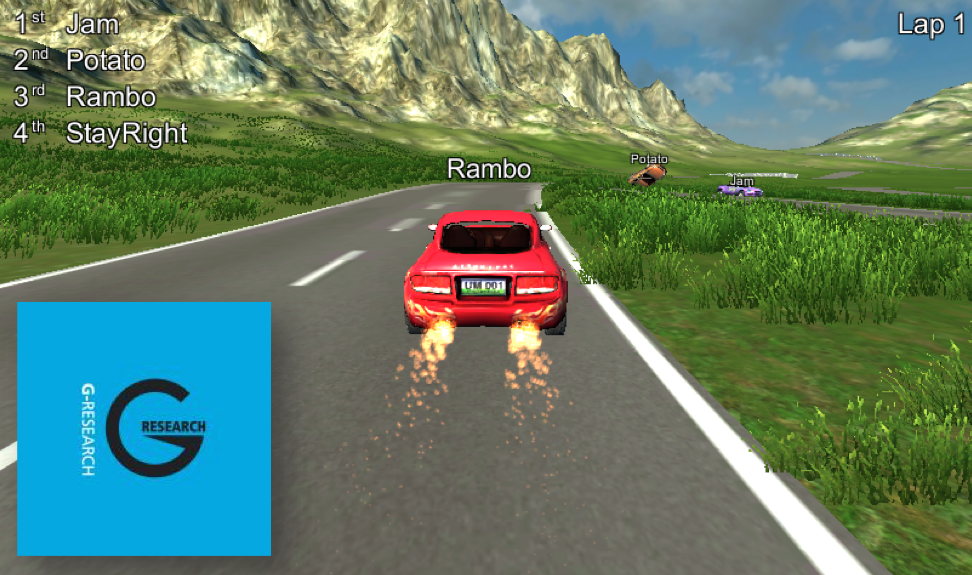
\includegraphics[width=0.9\textwidth]{coverpic.png}}
}
\author{Christophe Steininger, Finlay Curran, Jaime Lennox,\\ Ben Lindsey, Louis Mackie, Thomas Kaplan}

\begin{document}
\maketitle

\chapter*{Executive Summary}
Remember: No implementation details, engineering details or project management.

\section{What is our project?}
Our task was to create an AI racing market - a platform for users to submit racing algorithms in a driving simulation that would be rendered with the Unity engine. In the future, algorithm markets could be applied in other problem domains (e.g. in finance).

\section{Who is our customer?}
This project is co-supervised by G-Research, a financial services company that evaluates, forecasts and simulates investment ideas across multiple financial asset classes. They produce software and services across a range of markets, allowing the deployment of these investment ideas and portfolio risk management.

\section{What does it do?}
\section{Why use it?}


\tableofcontents

\chapter{Introduction}
\section{Motivation}
Careers fairs are designed to be an exciting opportunity for companies and students to interact and learn about each other. Ideally students will gain an understanding about various career sectors that they would be interested in working in, and advice to assist them in their application from employees who are working in specific companies. Well prepared students might have a few companies that they particularly want to meet to network with and improve their chances of an offer. However, in practice for many students attending, careers fairs involve picking up a dozen leaflets and free pens, eavesdropping on conversations and perhaps sidling up to a quiet stall and asking a recent graduate ``What exactly does your company do?''.\\

From the perspective of a company attending the fair this is also an issue. If they aren't engaging with students attending the fair, how can they give them personal advice on their CV? How can they meet with the brightest students and personally encourage them to apply? How can they explain to students why their company is such a great place to work?\\

G-Research, who attend careers fairs at Imperial and various other universities would like to improve the experience for students they meet.  There are two key challenges for companies in the recruitment process:
\begin{itemize}
	\item Generating interest from potential applicants
	\item Evaluating aptitude of candidates
\end{itemize}
By having a more exciting stall G-Research would attract more attention during the fair which could lead to more enthusiastic discussion, or at the very least instigate some Google searches from students later that evening. Some companies use quizzes during career fairs, perhaps to serve as a fast-track through the recruitment process for particularly promising individuals. G-Research's idea to improve their stall is this project - the AI Racing Market. This solves the two challenges above, as it would be a fun activity which students should be enthusiastic about getting involved in, and the competitive aspect of the game will allow smart candidates to excel. Additionally employees present will be able to interact with the players as they are writing code, giving a glimpse for both of them of the day to day software engineering environment at G-Research.
\section{Objectives}
Our objective was to create an AI Racing Game using the Unity framework that allows users to design an AI to race a car around a track.

Our initial project plan we developed with consultation and approval from Ed Cresswell, our supervisor from G-Research, specified a minimum viability product that could be used at a career fair.

\begin{itemize}
	\item Website interface
	\item Web server runs on G-Research's Windows laptops
	\item Users watch their AI race in real-time using Unity
	\item Users can design scripts using a simple editor on the website
	\item Scripting language should be intuitive enough for a new user to develop a simple AI in a few minutes
	\item Scripting language should have enough depth for experienced users to develop more complicated AIs
	\item Users have accounts which save scripts they have written
	\item Users can fill in personal information visible to G-Research employees (Name, E-Mail, Degree)
	\item Users can edit their saved scripts
	\item Multiple cars can race against each other
	\item Database tracking some performance metrics of races
\end{itemize}

The simplicity and depth of the scripting language would be one of our key objectives. At a careers fair stall with high turnover a user with some programming knowledge should be able to develop a simple AI within 5-10 minutes. Our vision was that a simple script that kept in the middle of the track with constant speed could be implemented in a matter of seconds. However, to race AIs against each other there would need to be enough depth to support meaningful design choices from users that allow their scripts to beat others. Another possible use case for the project is as part of a larger event, perhaps taking place over 2-3 hours where teams try to develop advanced scripts.

Once we had our product we met with Ed and discussed some extensions we would like to implement.

\begin{itemize}
	\item Increased API depth
	\item Elo rating system
	\item Testing scripts against a practice AI
	\item Unity HUD
	\item Iterative testing environment for scripting
	\item Scripting API access through Javascript
	\item Multiple tracks to race on
\end{itemize}

\section{Achievements}

The minimum viability product was finished quite quickly, giving us ample time to focus on our extensions to create a great user experience. We have done a test set-up on a G-Research laptop to ensure they can run the project.

\subsection{Profile}
\centerline{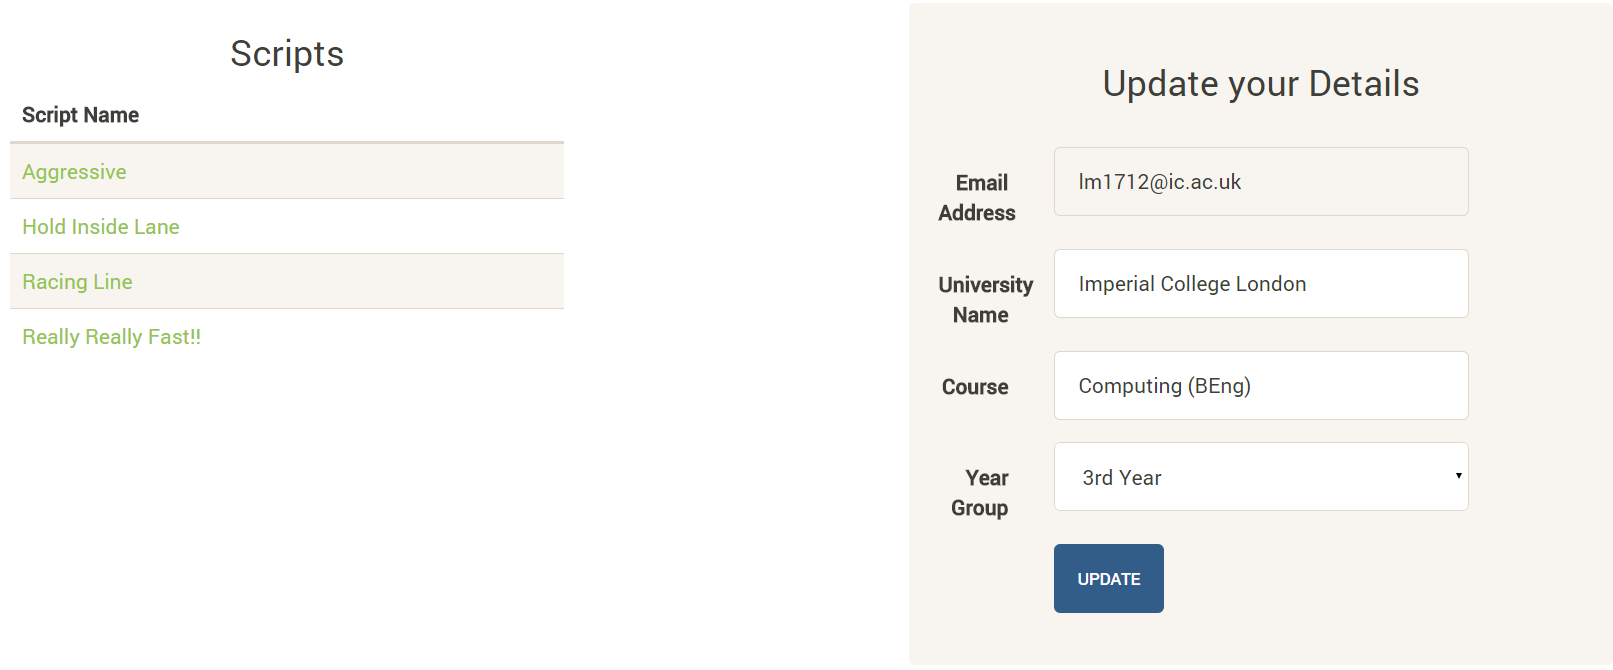
\includegraphics[scale=0.34]{profile}}
User accounts store some optional personal information interested students can fill in. The scripts on the left hand side of the page are owned by the user and can be edited at any time. The admin user can view these details, and see who owns which scripts.

\subsection{Scripts}
\centerline{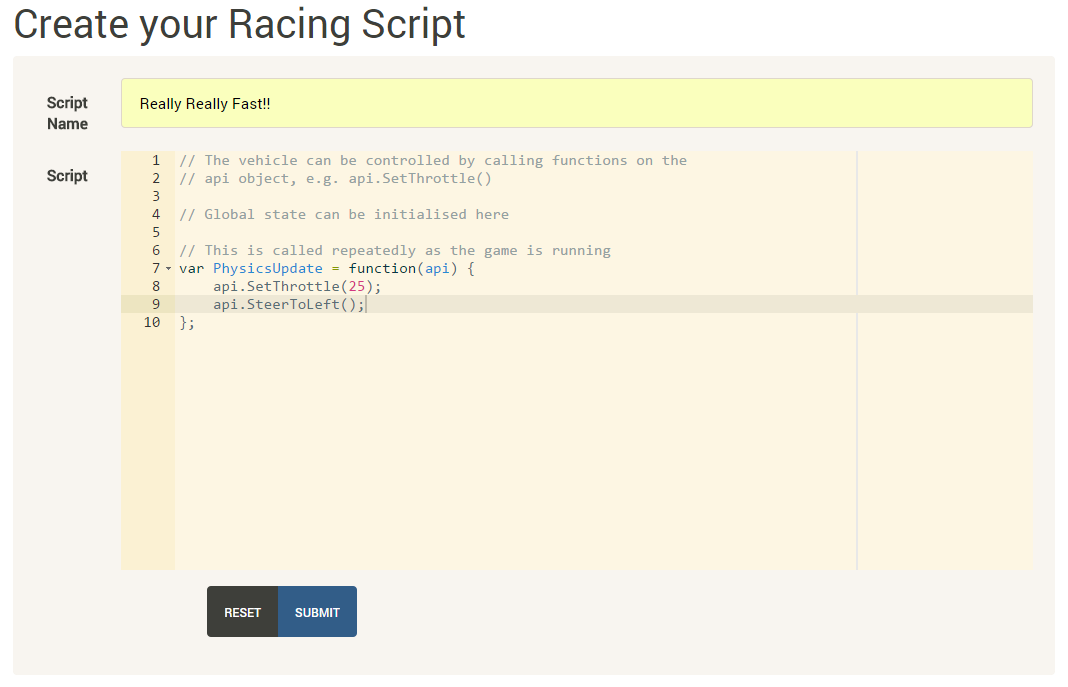
\includegraphics[scale=0.5]{script}}
Scripts can be written in either Coffeescript or Javascript and are very easy to code. Above is a trivial two line script which can be implemented in seconds, and will drive around a track at a constant speed holding the inside lane. There are many more API calls available to design superior scripts with greater complexity, such as using boost, getting proximity of nearby cars, and the determining sharpness of the next corner. Full API documentation is available in appendix A. While editing scripts users can run test races to see how their AI stacks up against others, and to get quick feedback on any changes they make.

\subsection{Races}
\centerline{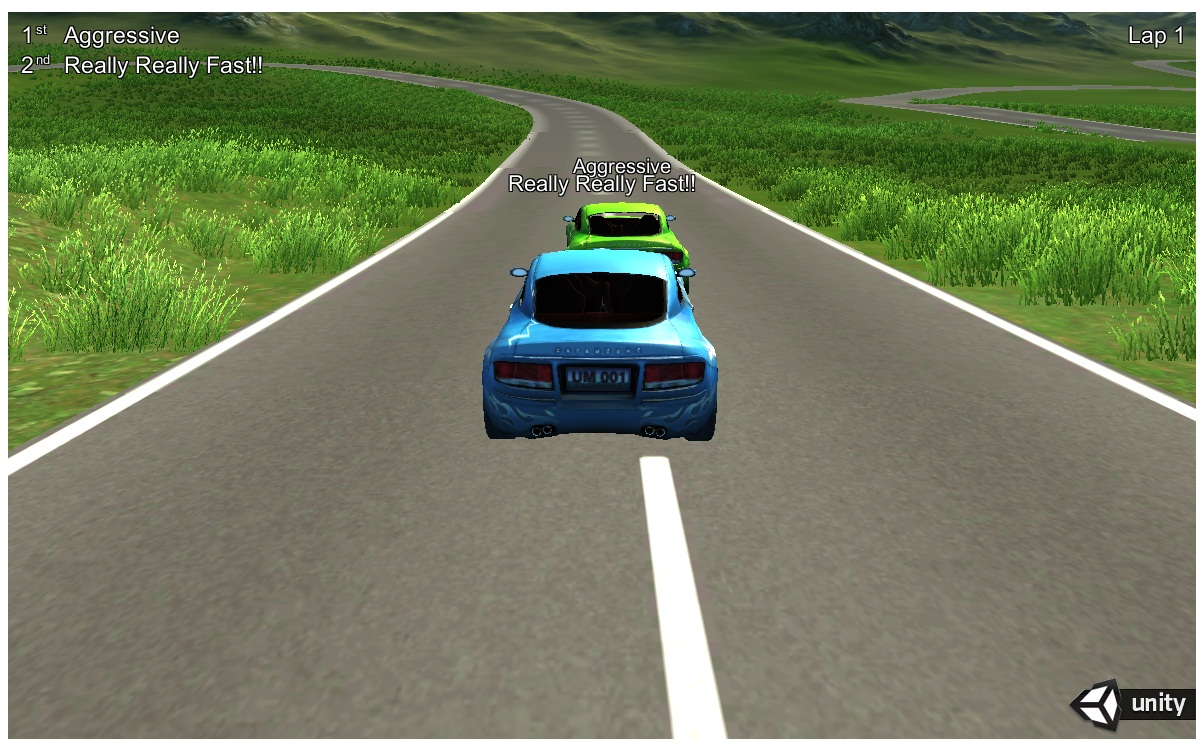
\includegraphics[scale=0.5]{race}}
Creating races allows for a variety of options, including different number of cars and a choice of multiple tracks. Once options have been selected, the race is run in Unity and the users can cheer their scripts on. The camera can move between the different cars and the HUD tracks the lap number and the positions of the cars. At the end of the race the results are sent to the database and the updated leaderboard is shown to the user.

\centerline{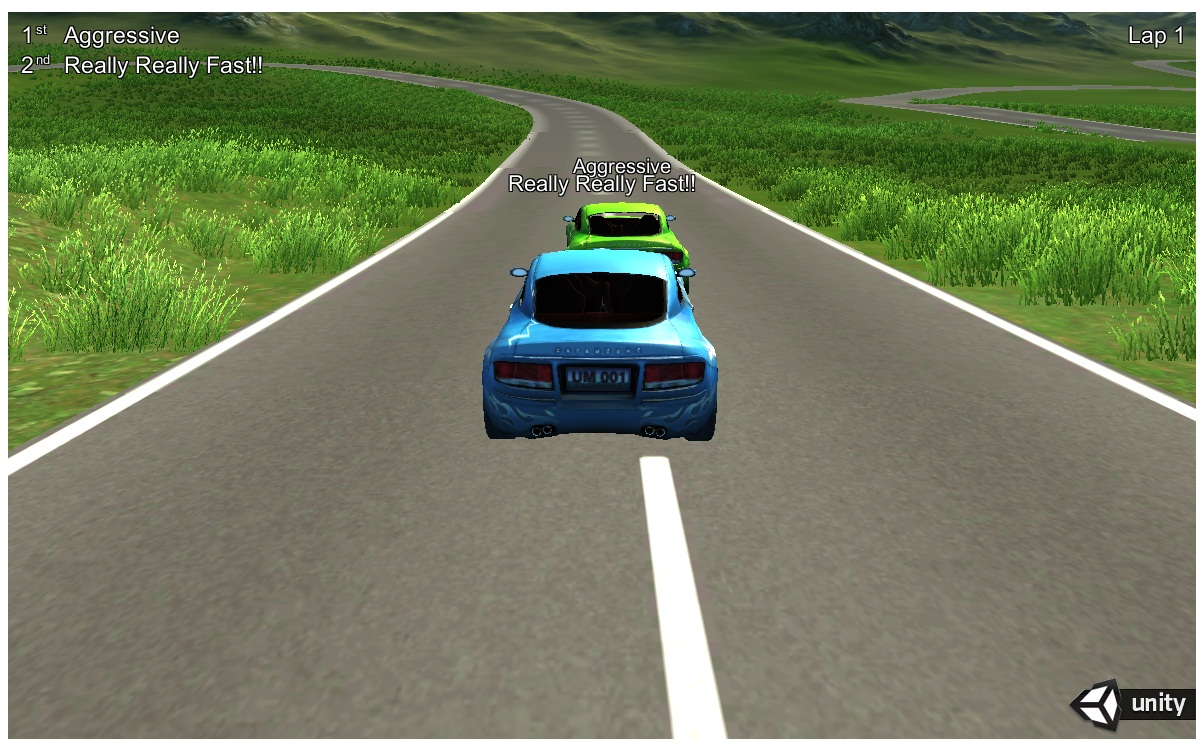
\includegraphics[scale=0.405]{race}}

\subsection{Leaderboard}
\centerline{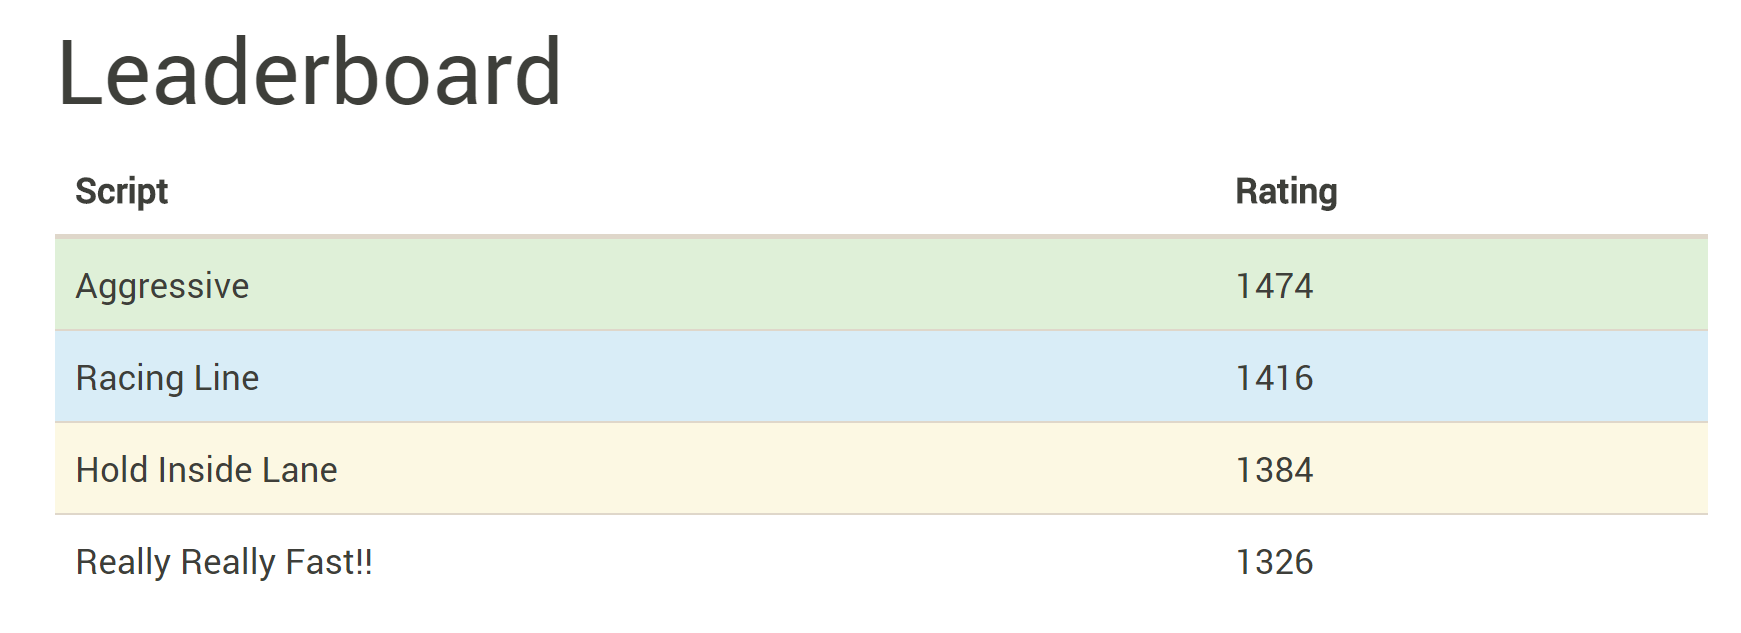
\includegraphics[scale=0.35]{leaderboard}}
A leaderboard displays the Elo ratings of each script, calculated after each race. With enough races the best scripts will rise to the top.


\chapter{Project Management}
\section{Software Design Methodology}
A large focus of this group project was using an Agile development approach, similar to the Scrum iterative and incremental process (see figure 2.1 below). The idea behind Agile is to maximise the flexibility of the development process and assist in communication. Wherever possible we tried to apply these concepts to our planning and the way that we worked. The Sprint system allows us to refocus our goals regularly and requires meetings to discuss progess. Excluding Sprint Zero, we had three week Sprints, starting on Mondays and ending on Fridays. Our Product Owner was Ed Cresswell from G-Research.  Ideally we would have liked to have shorter sprints but were limited by our product owner not being on campus. We chose to not have a Scrum Master and we used Trello instead of a physical task board.

\begin{figure}[H]
\centering
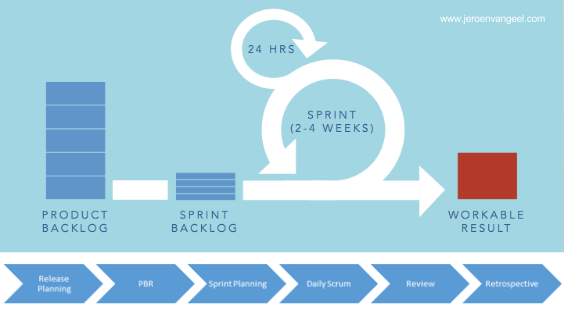
\includegraphics[scale=0.7]{sprint.png}
\caption{Scrum iterative and incremental process.}
\label{fig:scrum}
\end{figure}

Due to our Product Owner's busy schedule and the difficulty in having to travel to meet with us, we were only able to meet with him every 3 weeks for Sprint reviews following Sprint planning. We met on a regular basis in the college, but did not have a formal stand-up.

\section{Risks and Issues}
\subsection{Organisational}
Organisational risks we managed throughout the project:
\begin{itemize}
\item A limited number of meetings with our Product Owner made it difficult for them to communicate their requirements and consequently steer our development.
\item We over and underestimated our ability to deliver on the stories we committed to in a Sprint, due to inexperience working in a formalised agile environment.
\item Difficulty exposing every group members to all the technologies used. This limited communication within the team as not all team members were able to assist each other due to unfamiliarity with technology.
\item Of course, all team members had other commitments that conflict with this project's organisation, such as coursework, exams and job/placement interviews, which limited the time we could contribute.
\end{itemize}

\subsection{Ongoing}
Ongoing issues which we had to consider that would persist after we hand-off the product to G-Research:
\begin{itemize}
\item We are producing a product on behalf of G-Research, so there are questions relating to the final product shipping:
\begin{itemize}
\item G-Research pitched this same project to both Cambridge and Oxford.
\item G-Research want ownership of the project.
\item The project we developed had to be self-contained, it couldn't be tied to G-Research's software frameworks.
\end{itemize}
\item We ensured that the frameworks, libraries and resources we used have suitable licenses, considering that we developed the product for use in a corporate environment.
\end{itemize}

\section{Estimation of Work}
(mebbe dis goes above risks?)
Sprint Zero was an opportunity to gauge the rate at which we worked as a group, to assist in future estimation. We swiftly developed an entire slice of our software stack - we created a basic prototype to give us an idea of the difficulty of our planned features. For example, within a few days we created a car model in Unity that met our simulation requirements. Off the back of this we increased our product scope to include more elaborate car physics and expect to spend a lot of time on stretch requirements (e.g. multiple vehicle types and introducing powerups). This also influenced our thinking when estimating the size of future tasks. We expected that after Sprint Zero that physics work in Unity would take less time than we initially estimated.

We used story points as a metric to measure the amount of effort required to implement a story. These points are displayed on each Trello to easily differentiate major and minor tasks. As the project progressed, we compared the total story point difference between tasks planned and tasks completed in each Sprint. This indicated whether we under or overestimated our workload during Sprint Planning. As we have worked in numerous group projects together, we already had a rough baseline in our minds for estimating task size. We used this notion when assigning story points to tasks in our backlog.

\section{Creating a Plan}
The first day of our project began with a struggle - a serious lack of direction. We were given a short paragraph describing our task, and unfortunately that was all the instruction we had for two weeks of work. While most groups met with their supervisors within the first few days, our product owner was hard to reach as we couldn't contact him directly (Our group $\rightarrow$ Marc, Imperial contact $\rightarrow$ Emily, G-Research HR $\rightarrow$ Ed, G-Research product owner). Due to the difficulty in communicating with our product owner, we were unable to setup an initial planning meeting until close to our first deadline.  In fact, for our first week we were unsure if the meeting would occur at all.

So we were faced with a hard decision, should we hold off on development until we could form a plan with Ed, or carry on undirected? It was clear that both options had risks, if we coded our own vision it could be rejected by our client and result in a huge waste of our time. And yet, if we were to stall for that initial meeting we might have to keep pushing back our work until it was deadline night, whereby our work would be reviewed the next morning! Ultimately we chose to charge on unaided, believing some progress is better than none, which strongly influenced the evolution of our plan. 

A key component to the success of a group lies within its ability to stay self motivated. With the looming threat of our work being scrapped when our first meeting arrived, we delegated work by interest. Ensuring that everyone was coding parts they were excited to be coding allowed us to justify working hard even if the project went in the wrong direction and had to be scaled back.

Clients are well known for their sudden changes in requirements and wishes (and we hadn't even met this client yet) so our plan had to be flexible enough to handle just about anything. To maintain this flexibility we frequently discussed our progress, trying to place ourselves in G-Research's shoes and imagining what they would want us to achieve. Wherever possible we focused on work that had to be done regardless of a change in requirements. Tasks such as setting up the VM, installing development tools, and learning about technologies directly specified in the project description - such as Unity.

We began Sprint Zero with a short sighted approach to planning, focusing on what we could achieve today rather than working toward a long time goal. While this made sense before meeting our PO Ed, afterwards we had more of G-Research's goals in mind, specifically that we were designing our project to be used at a career fair. With this new insight we refocused our direction and aimed to simplify our API. This was one of the few changes we had to make after first meeting Ed, highlighting how successful we were in producing code unlikely to change in the face of changing requirements. Establishing the initial contact with Ed and being able to discuss what to focus our efforts on for each split made subsequent Sprints far simpler to plan.

\section{Tracking Progress and Managing Work}

\subsection{Agile}
To track our progress on this project we maintained a Product Backlog and Sprint Backlog. Our Product Backlog lists all of the features that the client requires in the final product, as well as some possible extensions. The Sprint Backlog tracks items that should be completed within the current three week Sprint, and are filled from the Product Backlog. The features with the highest priority in the Product Backlog were chosen first - these may be broken down into smaller tasks if a major feature cannot be implemented in one Sprint cycle. Splitting up larger features also made it easier to estimate the size of the tasks as well as making progress easier to track. As the Product Backlog was filled, individuals or pairs were assigned to tasks until all group members had a clear understanding of what they need to accomplish over the coming three weeks. Being able to see what individuals were working on at a glance ensured that no-one stepped on each others toes when developing.

Along with the Sprint Backlog, we maintained a Doing and Done list for tasks in a Sprint. This allowed us to check our progress of the current Sprint by glancing at which columns the tasks were in. We used this to adapt our work according to our other varying commitments and how fast we completed the tasks we were focusing on at the time - when Sprint tasks were being completed early we were able to add additional tasks partway throughout the Sprint.

Beyond managing our work, we needed to be adaptable- as listed in our plan, there were many organisational risks and issues which could affect the team's performance (e.g. inflexible roles) that we had to be mindful of. Having Sprint Retrospectives immediately after each Sprint Review allowed us to evaluate and improve our development process so subsequent Sprints could flow better. This was also a key moment where all group members could get together and discuss the current status of the project, considering that we all had various conflicts that led to our work times being disjointed. Any issues or improvements raised would then be added to Trello for the following Sprint.

\subsection{Trello}
We used Trello as a task board, creating cards for stories and checklists for tasks. Using the `Scrum for Trello' Chrome plugin, we were able to assign story points to each card and visualise progression on a burndown chart. We decided to use one board as opposed to a new one for each sprint for ease of maintenance and monitoring progression against the product backlog. We made use of labels to denote cards that are blocked, introduced late in a sprint (i.e. after planning) or not finished during a previous sprint. This proved to be useful during retrospectives when assessing how effective our planning was.

\subsection{Facebook Chat}
We also had a Facebook chat for our project, for simple communicating when working in a distributed manner. While Facebook chat is a fairly simple tool, it was especially useful for deciding when we want to meet up, or for quick discussions about project progress (e.g. bugs and other blockers).

\subsection{git}
As with all our project work at Imperial, we used git for our version control, hosting on our private Github repository. This worked well for group organisation and eases the handoff to G-Research, as they can clone our repository and be almost ready to go. Our use of branches over the course of the project worked well with our Agile development methodology, as each story in our Sprint could be handled on a seperate branch. This allowed stories to be focused on in isolation, no one elses code from other features can interfere with current progress. Additionally, any group member interested in the progress of a story can simply read the git logs for a branch and be up to speed with no clutter from other stories in development.

\iffalse
Since we using git for our version control, and Github as our host for the project, we made use of Github's in-built issue tracking system. (Currently we use Trello to flag up issues, sometimes breaking our task board story-system by making a new card just for the issue. Using a dedicated system could help organise what problems we are having, in particular which issues are preventing further work from being completed. However, Github's 'Issues' feature isn't just restricted to bug fixes; it can be used for enhancements and keeping track of who is working on what, so it might be worth using this as an alternative, or in addition to Trello.) (Did we even use this?)
\fi

\section{Team Roles}
TODO (Each person fills their own in like last time?)

\subsubsection{Louis}
ayy lmao

\begin{center}
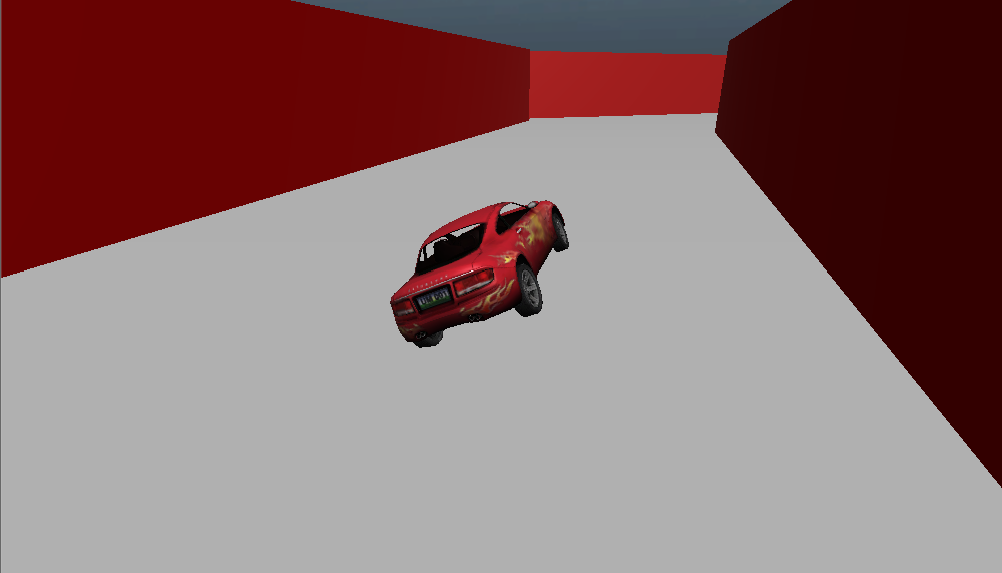
\includegraphics[scale=0.4]{prototype.png}
\end{center}


\chapter{Design and Implementation}
\section{System Architecture}

Our first step, after reading the description of our project, was to decide what kind of application or system would be best suited to tackle our requirements. The first thing that we gleaned from the specification was that some form of persistent storage would be required. For example, the user submitted scripts must be stored so that they can later be raced against new scripts and data used to rank the scripts must be recorded so that a leaderboard can be shown. It was also mentioned in our project's specification that we should use the Unity game engine for the physics simulation and visualisation of our vehicle races. These two requirements gave us a solid starting point for designing our system. Our first thought was to develop a stand alone Unity application to run on any desktop machine. This option would have required one machine to act as a server and manage the centralised data while the other machines communicate with it using networking code inside of Unity. It would also have meant we'd need to build a full user interface for uploading, editing and managing scripts inside of Unity. The more we thought about this the more we realised that these tasks would be a massive undertaking and highly difficult to achieve in the time frame, due to our group's limited knowledge of Unity.

Once we began thinking about alternatives an obvious solution sprang to mind. A huge benefit of Unity is that it is highly portable and can be run on many different platforms. One of these platforms is the Unity Web Player, a browser plug-in that allows Unity applications to be run inside all modern web browsers. If we used the web player we would could pull all of the things that are difficult to do in Unity outside of the Unity application and into the web browser. Thus turning the task of creating an easy to use interface for uploading scripts into a web design problem, a domain that is a lot better suited to solve user interface tasks such as this. The Unity application is then only needed for running and visualising the races. Unity also provides features for communication with the web browser, in both directions, when running in the web player, making passing data to the Unity application at runtime easy. This design also reduces the complexity of the networking problems as now one machine can run a web-server and database, using standard web technologies, while client machines simply run a web browser, containing the Unity Web Player, and communicate with the server using standard web protocols.

\subsection{Component Diagram}

\tikzset{%
  block/.style    = {draw, thick, rectangle, minimum height = 3em, rounded corners,
    minimum width = 3.5em, align=center},
  sum/.style      = {draw, circle, node distance = 2cm}, % Adder
  %input/.style    = {coordinate},
  db/.style  = {draw, cylinder, shape border rotate=90, aspect=0.25},
  interface/.style    = {draw, thick, rectangle,
    minimum width = 4em, align=center},
}

\begin{center}
\begin{tikzpicture}[auto, thick, node distance=2cm, >=triangle 45]
	% Blocks of FRONT END:
	\draw
		node at (1, -1.7) [block] (unity) {Game \\ Objects}
		node [block, right of=unity, right=-0.25cm] (webplayer) {Unity \\ Webplayer}
		node [block, right of=webplayer, right=-0cm] (unityscript) {Unity \\ Script}
		node [block, right of=unityscript, right=-0.35cm] (ai) {AI\\Script}
		node [block, right of=ai, right=-0.5cm] (browser) {Browser}
		%node [sum, right of=input1] (suma1) {Unity}
	;
    	% Joining FRONT END:
	\draw[->] (browser) -- node {} (ai);
	\draw[->] (ai) -- node {} (unityscript);
	\draw[->] (unityscript) -- node {} (webplayer);
	\draw[->] (webplayer) -- node {} (unity);
	\draw[-] (webplayer) |- node[right=3.5cm, above] {\small Request Commands } ($(browser.north) + (0, 0.5)$);
	\draw[->] ($(browser.north) + (0, 0.5)$) -- node {} (browser);

	% Blocks of MIDDLE
	\draw
		node at (5.5,-4) [block, name=rest] {REST API}
	;

        % Blocks of BACK END
	\draw
	        node [block, below of=unity, below=2.3cm, name=express] {Express\\Router}
	        node [block, right of=express, right=0cm, name=passport] {Passport \\ Auth.}
	        node [db, below of=passport, below=0cm, name=mongo] {MongoDB}
	        node [interface, above of=mongo, above=-1cm, name=monk] {Monk Adapter}
	        node [block, right of=passport, right=0cm, name=routes] {Routes}
	        node [block, right of=routes, right=0cm, name=views] {Views}
	;
	% Joining BACK END
	\draw[->] (express) -- node {} (passport);
	\draw[->] (rest) -| node {} (express);
	\draw[->] ($(browser.south) + (-0.2, 0)$) |- node[left=2.25cm, below] {\small Request Page} (rest);
	\draw[-, dotted] (passport) -- node[below right] {} (monk);
	\draw[-] (monk) -- node {} (mongo);
	\draw[->] (passport) -- node {} (routes);
	\draw[->] (routes) -- node {} (views);
	\draw[-, dotted] (routes) |- node {} (monk);
	\draw[->] (views) -| node {} ($(browser.south) + (0.2, 0)$);

	% Boxing
	%\draw [color=gray,thick, dotted] ($(passport.north west)+(-0.2,0.2)$) rectangle ($(monk.south east)+(0.2,-0.2)$);
	\draw [color=gray,thick](-0.5,-3) rectangle (12.55,0);
	\node at (-0.5,0) [above=5mm, right=0mm] {\textsc{Front-End}};
	\draw [color=gray,thick](-0.5,-10.5) rectangle (12.55,-5);
	\node at (-0.5,-10.5) [below=5mm, right=0mm] {\textsc{Back-End}};
\end{tikzpicture}
\end{center}

\section{Back-end}
The architecture of our server revolves around providing a website to upload, manage and score AI scripts. We provide these services via a simple REST API, implemented with Node.js\cite{whynode} and its supporting libraries:
	\begin{itemize}
	        \item \textbf{Express}\cite{express} is a light-weight web application framework that supports the MVC design pattern using routes (controllers) and views.  
		\item \textbf{Passport}\cite{passport} handles authentication for our website. We currently use the 'local' package which provides account registration and login via our Mongo database. However, in the future we could easily slot in Facebook or Google packages to provide alternative login methods.	
		\item \textbf{Monk}\cite{monk} provides a simple adapter to access our Mongo database in JavaScript. It uses an asynchronous tactic of searching by a filter object (e.g. to find a user called Steve, you'd filter with a new user object with name Steve) combined with a closure to be invoked on the found objects. 
\begin{figure}[H]
\centering
\begin{lstlisting}[language=JavaScript]
router.get('/script/:name', function(req, res) {
    db.get('scriptcollection').findOne({scriptName:req.params.name},  
        function(e, doc) { res.send(doc.script, 200); }
    );
}
\end{lstlisting}
\caption{Example use of Express (router.) \& Monk (db.) to GET a script.}
\label{fig:getscript}
\end{figure}
		
		\item \textbf{Forever} solves one of the main limitations of Node.js: that in the event of an exception the website will crash and shut down. Forever is a simple way to keep a script, and thus the website it controls, operating continuously. In the event of an uncaught exception, server restart or otherwise fatal condition Forever will restart the website immediately. Forever also maintains a log of such circumstances to help track down the cause.
	\end{itemize}

\subsection{REST API}
A Representational State Transfer (REST) design provides us with a stateless, cacheable interface for accessing our server. It unifies the various responsibilities of our back-end, such as providing webpages and updating script scores, behind a single vocabulary of HTTP requests:
\begin{figure}[H]
\centering
\begin{tabular}{| l | l | l | l |}\hline
Route & Request &  Response & Explanation\\\hline\hline
/script & GET & View & Show the create new script page\\\hline
/script & POST & None & Store a new script to the server\\\hline
/script/DrEvil & GET & String & Get the code for script DrEvil [see Figure \ref{fig:getscript}]\\\hline
/edit/DrEvil & GET & View & Show the live edit script page\\\hline
/tournament & GET & View & Show the next tournament match\\\hline
/tournament & POST & View & Store the match result and show the next \\\hline
\end{tabular}
\caption{Example interactions specified by our REST API.}
\label{fig:api}
\end{figure}

Figure \ref{fig:api} demonstrates the loosely-coupled nature of REST APIs. There are no inherant requirements placed on either the front or back end implementations. Our website could be accessed by a mobile or desktop device, while our server could be a local laptop, a VM cluster or a teapot\cite{rfc}. This allows us to update, or even completely scrap, either side of our architecture without having to fix the other.

\subsection{MongoDB}
For our database persistence we use an open source, document based solution - MongoDB\cite{mongo}. Mongo provides fast, scalable data storage with rich, object based queriers.

Our main motivation for using MongoDB was the flexibility its schema-less design offered\cite{whymongo}. Rapidly prototyping new ideas and concepts is much more productive when the updating and deployment of database schemas can be ignored. During such development data entries can frequently gain and lose attributes, which requires no interaction with the database when Mongo is used. Furthermore, by using the Monk adapter we can implement our full back-end in a single language, JavaScript, without complicated SQL statements.

\begin{figure}[H]
\centering
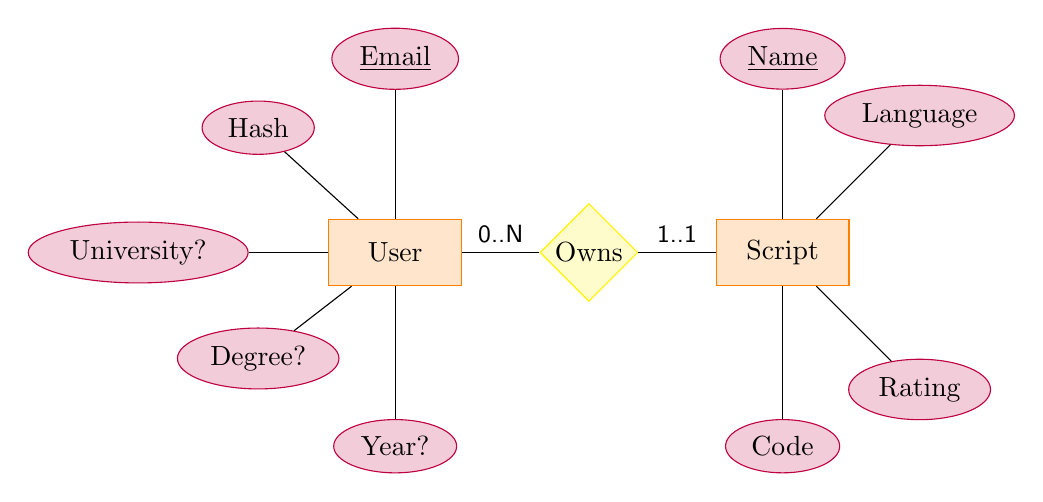
\begin{tikzpicture}[node distance=7 em]
\node [entity] (person) {User};
\node [relationship] (has) [right of=person] {Owns};
\node [entity] (script) [right of=has] {Script};
\node [attribute] (email) [above of=person] {\key{Email}} edge (person);
\node [attribute] (pid) [below of=person] {Year?} edge (person);
\node [attribute] (pid) [below left of=person, above=0cm] {Degree?} edge (person);
\node [attribute] (pid) [left of=person, left=-0.6cm] {University?} edge (person);
\node [attribute] (pid) [above left of=person, above=-0.5cm] {Hash} edge (person);
\node [attribute] (pid) [above of=script] {\key{Name}} edge (script);
\node [attribute] (pid) [below of=script] {Code} edge (script);
\node [attribute] (pid) [above right of=script] {Language} edge (script);
\node [attribute] (pid) [below right of=script] {Rating} edge (script);
%Edge
\path[every node/.style={font=\sffamily\small}] (person) edge node [above] {0..N} (has);
\path[every node/.style={font=\sffamily\small}] (script) edge node [above] {1..1} (has);
\end{tikzpicture}
\caption{ER diagram for our data persistence.}
\label{fig:ER}
\end{figure}

From Figure \ref{fig:ER} you can see another justification for our use of NoSQL technologies: the relationship is very simple. Document based technologies such as Mongo can struggle to provide simple modelling of complicated relationships, in these situations SQL based implementations typically offer a better solution. 

\section{Browser Front-End}

For the browser front-end, i.e. website, we used three technologies : Jade, Bootstrap and the Ace editor.


\subsection{Jade}
As explained above, we chose to use the Node.js platform, and we next had to chose a template engine for it's web template system. We chose to use Node's default engine, Jade\cite{jade}, which is written in JavaScript and specifically a templating language for HTML. It simplifies writing web pages as it is less verbose than HTML, and allows template inheritance (demonstrated below) alongside other dynamic constructs such as conditionals and loops.
\vspace{-2mm}
\begin{figure}[H]
\centering
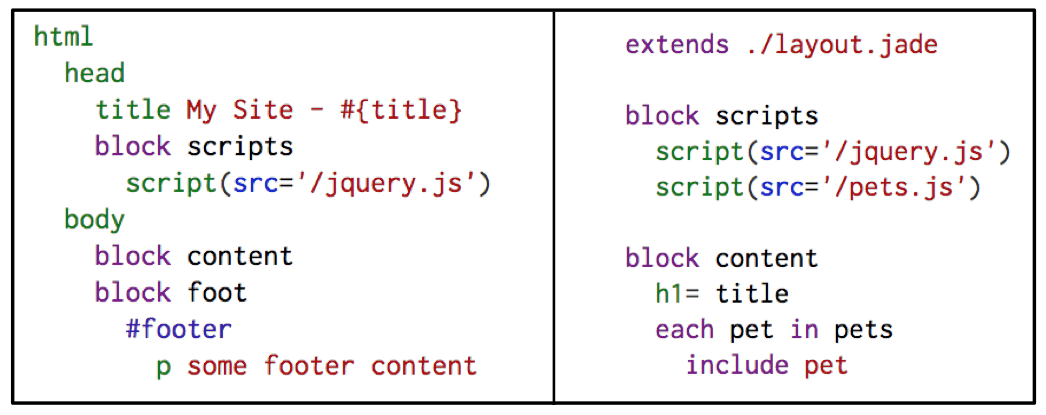
\includegraphics[scale=0.25]{jadeexample.png}
\caption{Jade template inheritance is simple and powerful.}
\end{figure}

\noindent Compared to other engines such as Swig and Hamljs, which have similar feature sets, Jade has had reported sluggish benchmarking performance \cite{benchmarks} (obviously some benchmarks can't be treated as gospel). However, performance was not a concern for us; templating engines are very rarely a system bottleneck, and the decision to use Jade was founded upon it's usability and readability.

\subsection{Bootstrap}
Given our limited experience using Jade/HTML and CSS, alongside our negligible artistic talent, we opted to use Twitter's Bootstrap to design our website. Bootstrap makes web design a breeze by providing the HTML and CSS templates for well-designed web components, including forms, buttons, navigation bars, JavaScript extensions and more. In particular, we used the Sandstone\cite{sandstone} template from Bootswatch (released under MIT license), demonstrated in the figure below. Although this may not give users with a particularly unique experience, it means providing users with a familiar experience that would allow them to utilise preconceived assumptions on how the website can be navigated - avoiding the need to explain the website explicitly.

\begin{figure}[H]
\centering

\includegraphics[width=0.5\textwidth]{sandstonetheme.png}
\caption{Bootswatch Sandstone theme sample.}
\end{figure}

\subsection{Ace}
Apart from the most cavalier advocates of text editors, programmers shudder at the idea of coding in a plain text area. To simplify the process of reading, writing and submitting scripts, we chose to use a web-based code editor. There are few open-source editors that can rival the performance, features and simplicity of Ace (a standalone editor written in JavaScript). Ace\cite{ace} is actively developed for use in the online Cloud9 IDE, yet can be embedded in any web page (see picture below) given its BSD license.

\begin{figure}[H]
\centering
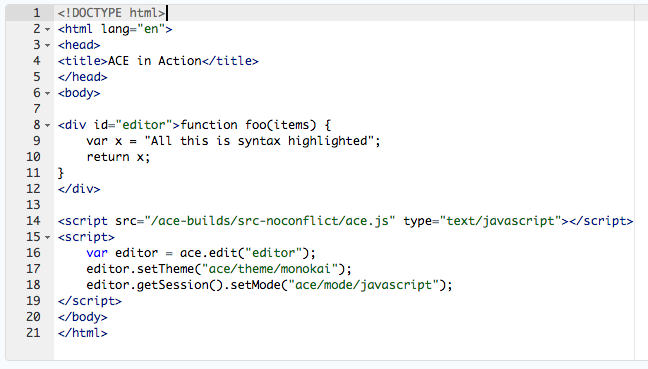
\includegraphics[width=0.75\textwidth]{aceeditorexample.png}
\caption{Ace editor containing code needed to embed in a web page.}
\end{figure}

\noindent By using Ace, users have JavaScript syntax highlighting, syntax error checking, searching/replace, automatic indentation etc. Not only does this improve the productivity of a user, which is important given the time pressures which may be faced if a queue forms at the G-Research careers fair stand; but it provides immediate feedback for those unfamiliar with JavaScript syntax, which may be the majority of users, reducing the likelihood of submitting broken scripts.

\subsection{Risks}

\subsubsection{Browser Cross-Compatibility}

It is rare for websites and web applications to function identically or appear the same across multiple web browsers, due to the varying compatibilities of even the most popular browsers - this can be problematic for many modern websites. We mostly spent time testing AI Racing Market on Google Chrome, yet tested on Mozilla Firefox and Safari occasionally. Needless to say, this does not replace proper cross-browser compatibility testing using the many tools (such as emulation environments) available to developers these days. However we did not deem this a significant risk, as G-Research employees should be able to iron out compatibility issues prior to a careers fair, installing and choosing the most functional browser in advance. With most of the well known browsers, it is likely that the user interface will simply appear jumbled yet remain functional.

\subsubsection{Mobile Compatibility}

Although users will not be able to run the game itself from a mobile device, it may be possible for students to submit their AI scripts from mobile devices at a careers fair (assuming G-Research permits it, given they will be hosting a local network). This could reduce queues for workstations at the stand. Unfortunately we did not develop our website with mobile users on mind, and some website components are coded such that they would perform poorly on small-resolution devices. This means there is a considerable risk of poor compatibility on mobile devices, that could greatly detract from a mobile user's experience. For example, the Ace editors do not resize gracefully, and as a result the user may struggle to view their scripts with full line width.

\subsection{Challenges}

\subsubsection{Streamlining User Interactions}

To prevent queues to play AI Racing Market at the G-Research stand, we focused on minimizing the user interactions needed to reach the script submission screen. As we were inexperienced web developers at the start of the project, we relied heavily on Bootstrap to provide web components, hence were limited in how unique the user experience could be. Compared to any bespoke solution, using an off-the-shelf alternative (Bootstrap) posed the challenge of ensuring we could design an intuitive website. We describe our design philosophy and how we tackled this challenge in the User Interface Design section, later in this chapter.

\subsubsection{Unity Web-player Loading Times}

The majority of our website was lightweight, with simple components and little dynamic content. However, the Unity web player (which runs and displays the racing), loaded slowly and can occasionally freeze somebody's browser. This is largely out of our control, and we faced the challenge of ensuring a smooth user experience. When running a multiplayer race or a tournament, the user will be waiting for the race to start, and simply waiting for the Unity web-player's loading bar to fill. However, on the edit screen (described later in the User Interface Design section), the user is presented with not only the web-player, but an Ace editor, so that they can make changes to their script and get immediate feedback. 

It was clear to us that we had to avoid re-launching the Unity web-player when the user made changes to their script, as this could potentially freeze and crash someone's browser before they are able to save their updated script. This meant we had to run the Unity web-player in the background, or alongside the editor. We chose to run the web-player underneath the editor for two main reasons: computers with a large screen resolution will be able to view both their script and the editor, creating a more responsive editing experience; and the obvious approach to hiding the Unity web-player without restarting it was minimizing it to a 1x1 pixel resolution, however this resulted in Unity engine errors when initialising the web-player, making the approach infeasible. 

\section{Unity Application}
The Unity application is given the script names for each car and the track to use from the browser as well as the game mode of the race which determines what the application will do at the end of the race:
\begin{itemize}
  \item \textbf{Test Mode} used when editing a script. Creates an endless race which may be restarted by the user at any point.
  \item \textbf{Multiplayer Mode} used when manually setting up a race. The race will end normally and update the leaderboard. The user will be redirected to the leaderboard page at the end of the race.
  \item \textbf{Tournament Mode} only used during tournament races, this mode is similar to the multiplayer mode, but the user will be redirected to the next race instead of the leaderboard.
\end{itemize}

\subsection{API Design}
The key component of the Unity application is the scripting API and our first step in its design was to decide how to give information about the race track so the user can complete a lap. We eventually settled on making this very simple for the user - we drew a line along the centre of the track and let the user set the speed of the car. Our API will automatically steer the car along the centre line at the set speed. Our reasoning on making steering so simple was that guiding the car around the track is the first and least interesting step and we did not want every user to spend the first few minutes writing the same line following script. However this caused races to disintegrate into a train of cars following the same line around the track where the car in first place at the start of the race will be the winner. We solved this creating two more lines for the cars to follow on either side of the centre line and providing API calls to switch to the line on the left or on the right. These calls can be used to overtake cars or to switch to the inside line of a corner.

Finally, we added a few more features which scripts can use to distinguish themselves: the distance to the next corner, the curvature of that corner and a ``boost'' ability which gives the car a large speed increase but may only be used every few seconds. A good script can make use of these features by boosting along straight sections and slowing down according to the sharpness of the corner.

\subsection{Risks}

\subsubsection{Experience with Unity}
Most of our team was inexperienced in the Unity game engine; this posed a potential issue since it could hinder our development time while everyone learns the engine's workflow and quirks. However, a good part of these projects is learning new tools and technologies and if we had all used it before then we wouldn't really be learning anything new. Thankfully, one of our team members had previously used Unity and so could quickly explain how things work and the best practices to follow.

\subsubsection{Artwork and Models}
As computer scientists, creating good looking graphical models isn't really our forte. None of us had any previous 3D modelling experience either, yet this project required a 3D graphical racing simulation to be shown to the user. Whilst we could probably have developed some assets ourselves, if absolutely necessary, we quickly realised that learning to use 3D modelling software from scratch would have been a huge undertaking. As well as this, none of us have any notable artistic ability so we decided that doing it ourselves would have taken a huge amount of time and resulted in a sub par end result. Luckily for us, there is a large Unity community that provides many assets on the Unity Asset Store for use by anyone. These assets are all distributed under the same licence\cite{unityassetlicence}  which allows them to be used as ``incorporated and embedded components of electronic games and interactive media", for both personal and commercial purposes. This allowed us to use free downloads from the Asset Store for all our visual and audible assets, including the car and terrain models.

\subsubsection{API Depth}
The aim of the scripting API is to be complex enough to allow for a wide range of scripts and give users good control over the car, but simple enough to learn and use within 5-10 minutes, so we faced the risk of creating an API which did not find a balance between the two. In an early meeting with Ed, we decided we could mitigate this risk by designing API functions for both extremes where the simple functions alone should be enough to create a good script and users with more time could extend these scripts by using the complex function set. The simple function eventually included switch lane and set speed, while the complex functions included boost and distance to next corner. We also included the event based API to help users with very little programming experience as these scripts will resemble instructions in English.

\subsection{Challenges}

\subsubsection{Steering the Car}
To guide the car around the track we initially placed invisible walls along the edge of the track and created proximity sensors on either side of the car to measure the distance to these walls. The output of the sensors was used to steer the car toward the current lane. The main problem with this approach was that the cars would always drive forward even when pointing the wrong way after skidding or a crash causing the cars to drive the wrong way around the track.

\begin{figure}[H]
\centering
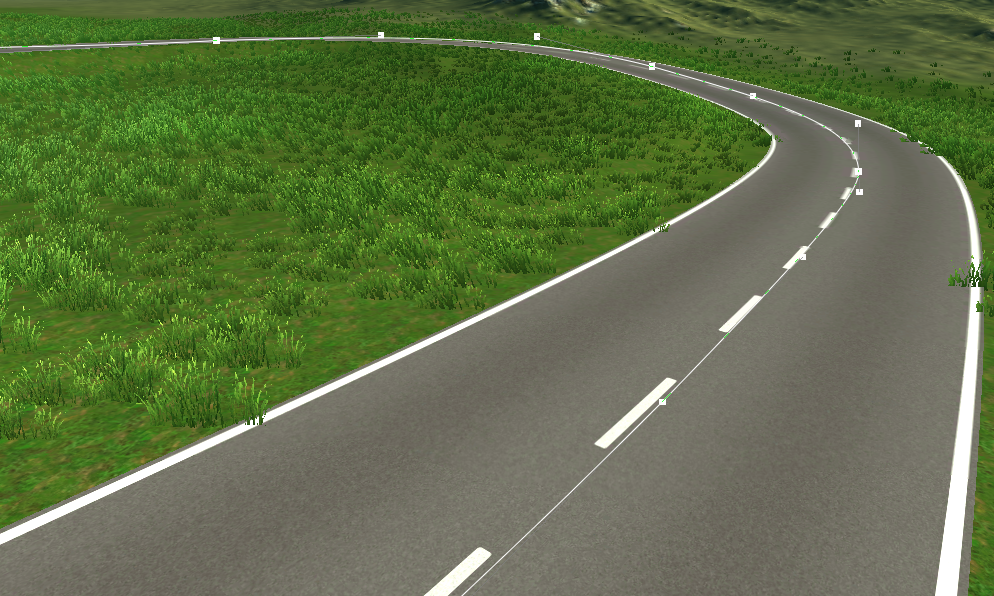
\includegraphics[width=0.75\textwidth]{spline.png}
\caption{The centre spline as seen in the Unity editor window.}
\end{figure}

We solved this problem by replacing the walls and proximity sensors with a spline along the centre of the track and keeping a target position on this spline. The car will always steer toward this target position and the target will always be a small distance in front of the car. This ensures that the car will always drive the right way along the track. Another advantage of the splines is that if two cars take a corner too quickly, the car moving faster will end up further from the track and therefore lose more time than the slower car. With the old approach, both cars would simply bounce off the walls and the faster car would not be penalised more than the slower car.

\subsubsection{Tournament Closing Conditions \& Ranking}
% Define "ranking of the cars" for the reader?
Users are able to submit scripts which cannot finish a race in a reasonable time or which will never finish e.g. cars which flip over in corners, cars which only drive backwards or stay at the start line and cars which override the default steering and go off track. So our tournament must be able to terminate a race before all cars have finished if necessary and still provide a good ranking of the cars.

\begin{figure}[H]
\centering
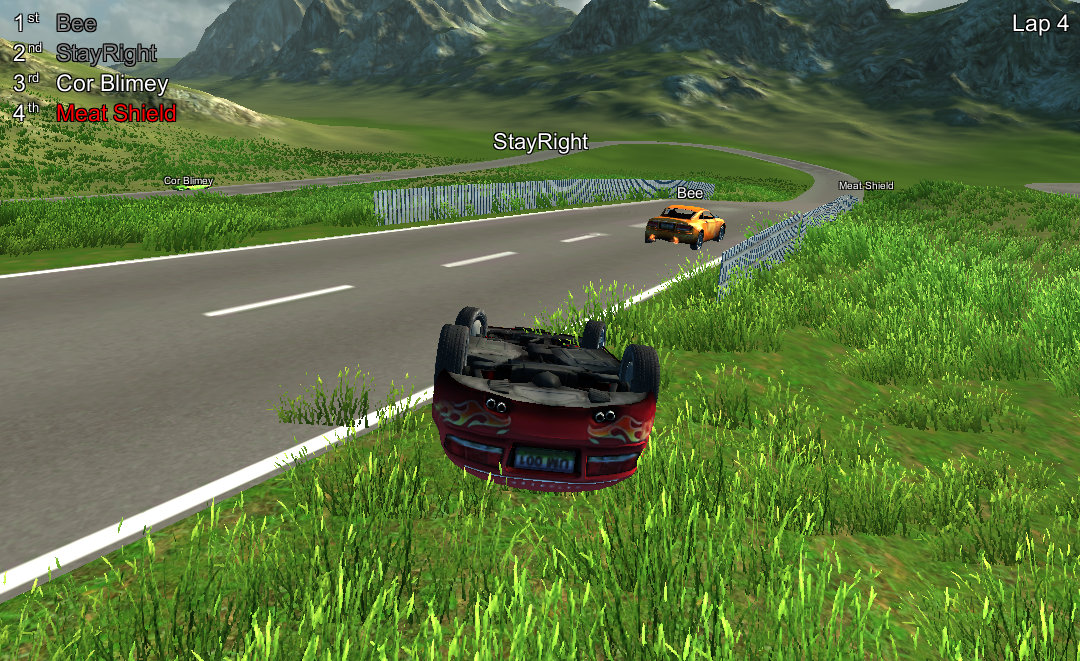
\includegraphics[width=0.75\textwidth]{HUD.png}
\caption{Cars which have completed the race are shown in grey, cars which have timed out are in red.}
\end{figure}

We accomplished this by placing invisible checkpoints to split each track into short straight sections. We keep maintain the next checkpoint and the time since the last checkpoint was completed for each car. From this we can tell if a car has finished (when the last checkpoint in the race is completed for the third time) or if the car has timed out (if the last checkpoint was completed more than 30 seconds ago). The 30 second time limit is very generous and even a cautious script can easily complete each checkpoint in this time, so a car which times out will belong to an incorrect script. The tournament is ended when all cars have either completed the race or have timed out. Cars which completed the race will be ranked by their time, while cars which have timed out will be ranked according to the number of checkpoints completed, if this is equal, the straight line distance to the next checkpoint is used instead.

\section{User Interface Design}

\subsection{Design Philosophy}

At a a busy careers fair we expect students will have roughly 5-10 minutes sessions with AI Racing Market. Ideally students will have the chance to return and improve their scripts, yet this may be infeasible if there are a lot of interested students. Given students will be short on time, under pressure and likely new to the game, we focused on :
\vspace{-1mm}
\begin{enumerate} \itemsep -2pt 
\item Simplicity
\item Minimal Interactions
\end{enumerate}

We previously justified our use of Bootstrap by the provision of a familiar user experience. By providing the user with a simplistic and familiar interface, users need little explanation of website navigation and can simply focus on script editing and submission. 

An example of how we achieved this was a common navigation bar seen on each web page. This functions as a website backbone, providing the user with access to all of the website's  features. Our template engine, Jade, made this incredibly simple (as shown below); we wrote a basic navigation template that extended our generic Bootstrap layout, which could then be included within the other templates (in Node.js, these are called {\it views}). 

\begin{figure}[H]
\centering
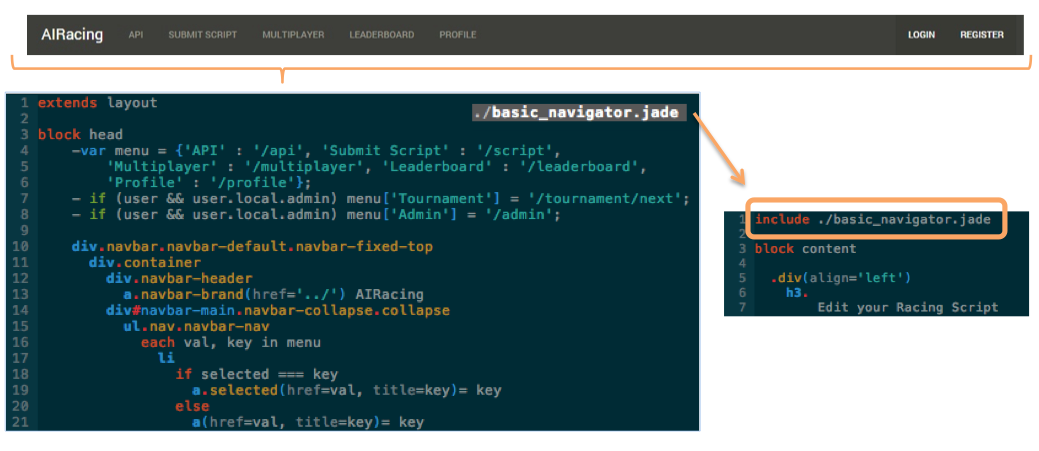
\includegraphics[width=\textwidth]{jadenavigator.png}
\caption{Jade navigator template included within each view.}
\end{figure}

\subsection{Anonymous Script Submission}

Few things kill the excitement of a new game like a lengthy registration process, especially when handing over your email could spell nothing but more email spam. Although we trust that G-Research wont spam students using AI Racing Market, or sell their email addresses to third parties, we designed the script submission such that the users did not have to register. Not only does reduce the interactions needed for a new user to get involved with racing, but it allows the users to remain anonymous, removing the concern that a poor performing script tied to their email address will result in G-Research immediately dismissing their application. As shown below, the user simply associates their work with a script name, and can immediately create a script.

\begin{figure}[H]
\centering
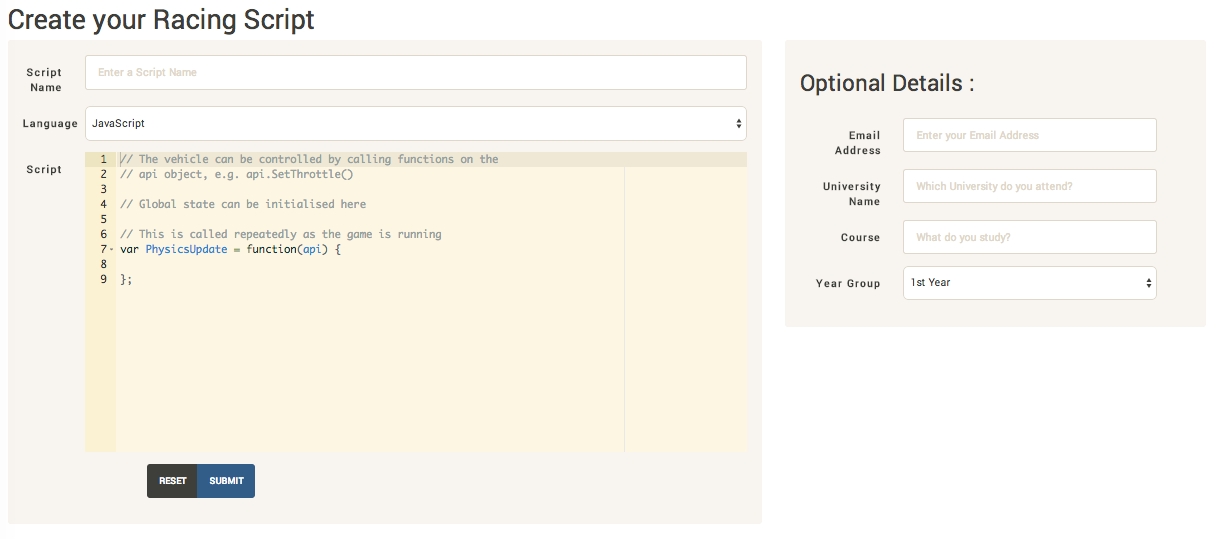
\includegraphics[width=0.8\textwidth]{anonymoussubmit.png}
\caption{Admins will see additional features on their navigation bar after logging in.}
\end{figure}

As we discuss later in this section, G-Research wants to harvest user data.  Therefore we added an ``Optional Details" panel on the right hand side of the script submission screen, allowing users to provide G-Research with information if they wish. If these details are submitted, they are not tied to an account or script until a user registers with the same email address. This means G-Research can recognize that a student has attended their careers fair stand, however their performance can't be scrutinised. If a user is already logged in and wants to submit a new script, they will face the same screen as shown above, excluding the optional details pane.

\subsection{Responsive Script Editing}

Clearly the script submission screen presented above is limited; it provides basic syntax checking, however users will have no feedback on how their scripts perform prior to racing in the tournament. If a user has registered, they can navigate to a more responsive editing mode by clicking on of their submitted scripts, listed on their profile (shown below).

\begin{figure}[H]
\centering
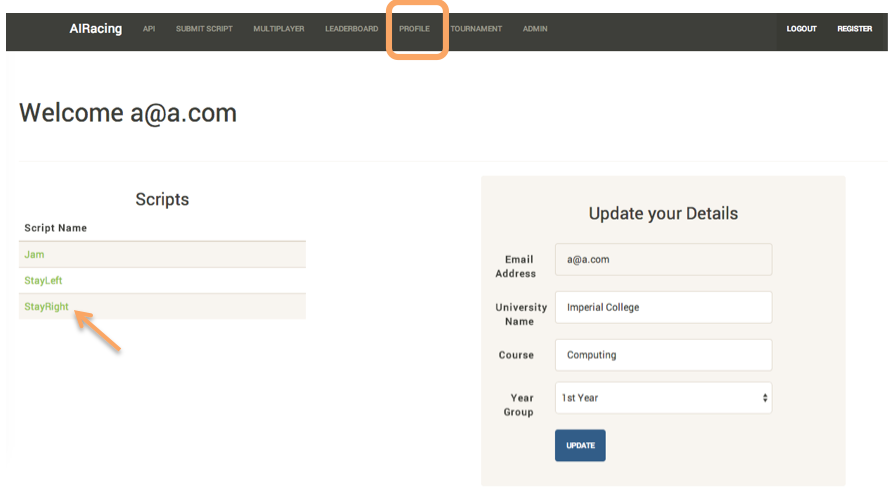
\includegraphics[scale=0.35]{profiletoedit.png}
\caption{Registered users have their scripts listed on their profile, these can be edited on click.}
\end{figure}

After selecting a script to edit, they are presented with not only an Ace editor, but a test race (shown below). Although the user cannot choose the car and track they test their scripts with, they can practice against an opponent script of their choice (without altering the leaderboard rankings). This allows for a more efficient and iterative development process, as the immediate responsive feedback to changes allows the user to incrementally improve their script. To improve usability, the script editing screen is incredibly similar to the script submission screen. 

\begin{figure}[h]
\makebox[\textwidth]
{
	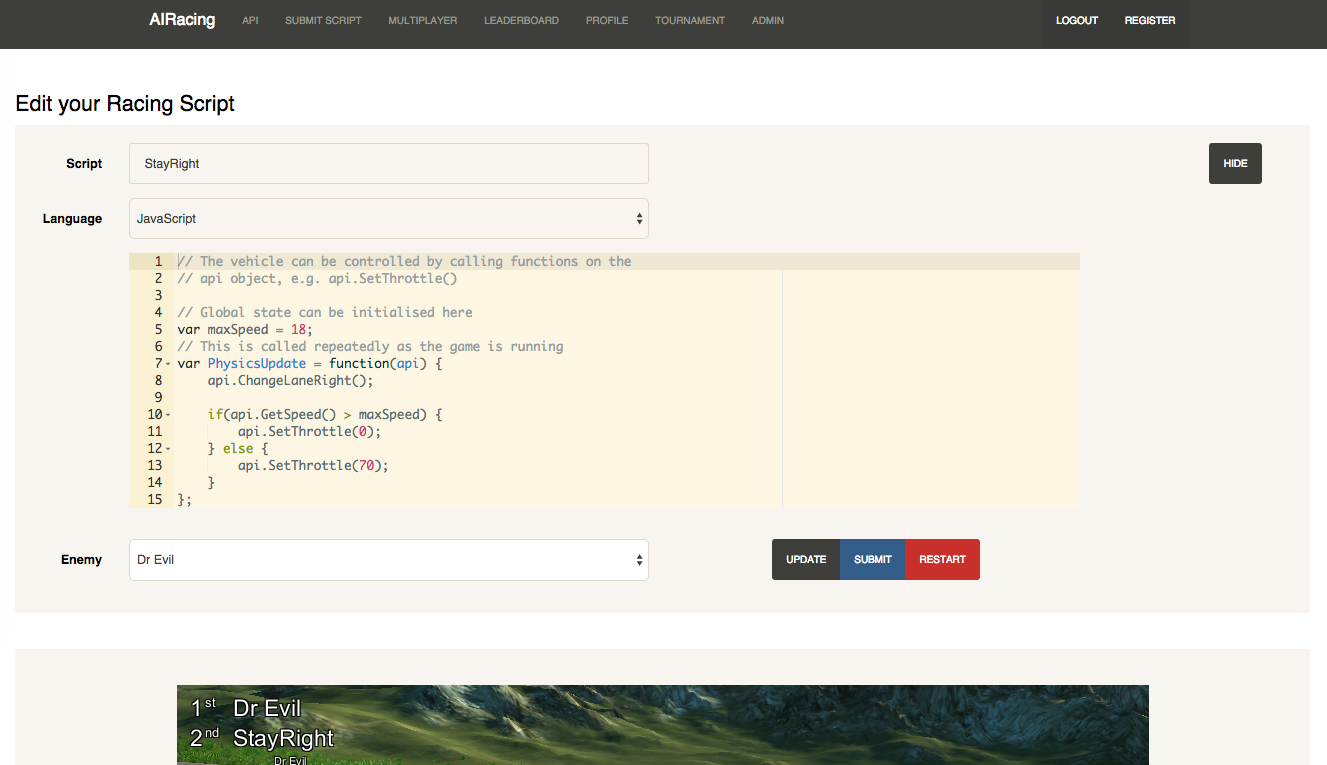
\includegraphics[width=0.49\textwidth]{editscreen.png}
	\hfill    
	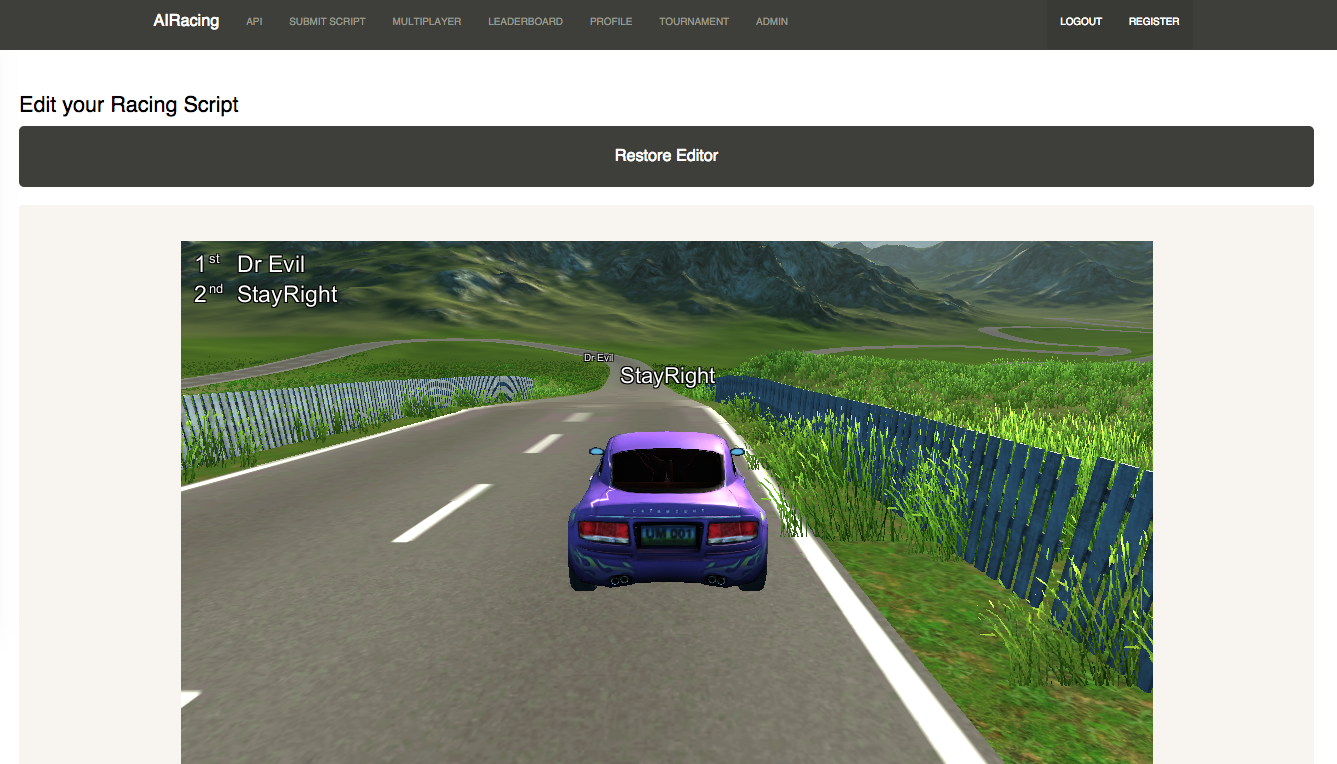
\includegraphics[width=0.49\textwidth]{editscreenhide.png}
}
\caption{Edit Screen - users can edit their scripts and test any changes made.}
\end{figure}

There are a few key differences between the script submission and editing screen, beyond the rather obvious Unity Web Player :

\begin{enumerate}
\item Hide button - Now that the user can also view their script racing alongside the Ace editor, we provided a hide button which allows the user to collapse the editing pane, displaying the race without forcing the user to scroll down the page. We decided not to display the race alongside the editor on the screen, as this either requires an unrealistically wide screen resolution, or would reduce the size of the editor and Unity web player drastically. We tested the edit screen using tabs, with the editing pane on one and the race on the other, however we experienced issues resizing the  Unity Web Player and running it in the background.
\item Restore button - After the editing pane has been collapsed, a large restore button is presented where the pane previously was. This is large to ensure that a new user does not accidentally hide the edit screen, struggle to restore it, and consequently leave the page without submitting changes. We could have used a more subtle restore button, and a  pop-up to notify the user of how to find it, but we did not want to obscure the Unity Web Player.
\item Update/Submit/Reset buttons - These new buttons are clustered together in the bottom right of the editing pane, below the Ace editor, to ensure they are visible when the computer being used has a small monitor resolution or if the web-browser has a high zoom level. Although clustering these buttons risks users accidentally submitting changes, we ensured the buttons had contrasting colours to avoid confusion.
	\begin{enumerate}
	\item Submit button - As the user is logged in, submitting changes updates the user's script and returns them to their profile. They are greeted by a pop-up that notifies them that their changes had been made successfully.
	\item Update button - Pressing the update button re-interprets the script, whether changes have been made or not. This allows the user to observe changes on demand, without restarting the race. 
	\item Reset button - Pressing the reset button restarts the race, re-interpreting the script and changing the opponent to the one selected in the ``Enemy" drop-down menu.
	\end{enumerate}
\end{enumerate}

\subsection{Admin Features}

We restricted a few features from the average user, which are only accessible by a registered admin, i.e. G-Research employee. These features were the tournament mode and admin panel, as shown below.

\begin{figure}[H]
\centering
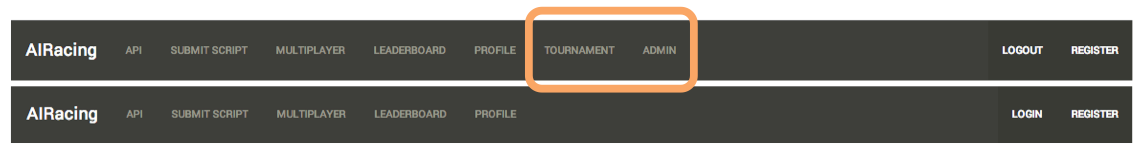
\includegraphics[width=\textwidth]{admintoolbar.png}
\caption{Admins will see additional features on their navigation bar after logging in.}
\end{figure}

These REST end points {\tt/tournament} and {\tt/admin} aren't secured from other users or anonymous users, however we do not expect users to access these features. This is mostly because users will be supervised by G-Research recruiters, but also because users will simply not know the names of these routes, and could only access them by trial and error.

The tournament button on the navigation bar will display a tournament, with races being run automatically with the leaderboard changes being displayed after each race. The admin button displays the personal details of registered users and the names of a user's scripts (shown below) - this feature was requested by our client. 
\begin{figure}[H]
\centering
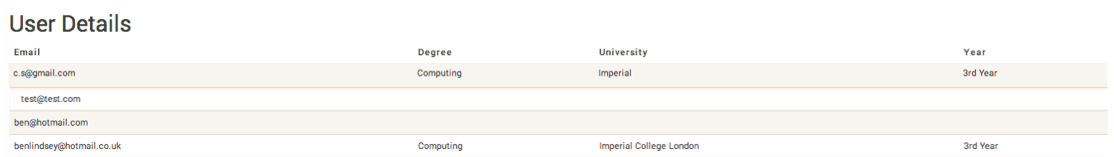
\includegraphics[width=\textwidth]{adminpanel.png}
\caption{Admins can view the details of registered users.}
\end{figure}

\section{Script Execution}
The architecture of our first prototype differed significantly from that of the final product. Originally, we required users to write their AI scripts in Unity Script - a bastardisation of JavaScript. These scripts were directly inserted into the Unity engine and executed on the car objects. While this design proved easy to implement, it offered some serious flaws:
\begin{enumerate}
\item Unity Script, while syntactically similar to JavaScript, has several key differences. For example, Unity Script does not offer the dynamic objects that are a core component of JavaScript. These differences would need to be taught to users.
\item Passing state between sequential executions of the script (such as, has a car recently been overtaken?) had to be done with a predefined global hash table. Users were unable to add their own variables to global scope.
\item Executing directly on a game object offers serious security concerns. Users with basic knowledge of unity could bypass our defined API and access the car's private data. Particularly cunning users could modify the car's x and y coordinates, teleporting the car to the finish line!
\end{enumerate}

\begin{figure}[H]
\centering
\begin{subfigure}{.5\textwidth}
  \centering
\begin{lstlisting}[language=JavaScript]  
global["speed"] = 20;

if(farFromCorner) {
  global["speed"] 
    = global["speed"] + 1;
}

\end{lstlisting}
  \caption{Unity Script}
  \label{fig:sub1}
\end{subfigure}%
\begin{subfigure}{.5\textwidth}
  \centering
\begin{lstlisting}[language=JavaScript]  
var speed = 20;

if(farFromCorner) {
  speed++;
}
\end{lstlisting}
  \caption{JavaScript}
  \label{fig:sub2}
\end{subfigure}
\caption{Comparison of prototype AI script and modern AI script.}
\label{fig:unityvsjava}
\end{figure}

To solve these issues we redesigned our front-end architecture by uncoupling the game object and AI script - replacing the direct calls with proxies. Now the AI script remains in the browser, never seen by unity, where it receives a serialised view of the game state and outputs a list of moves. This abstraction immediately solved (3) since the the proxy prevents any potentially dangerous requests like teleportation. 

Once a proxy had been defined the AI script could be in any language we choose, provided it handles the requests dispatched by unity. As the most popular web language, JavaScript is a natural choice for this - solving (1). Finally, now that the script is run in a JavaScript context, global variables can be easily stored in the browser window. Thus, the only problem remaining to solve (2) is isolating scripts global state (for example two scripts may both have a global "speed" variable, which should be sperate). We achieved this by binding each script inside a anonymous lambda, faking global state by using function local state.

Despite our protections there are still some flaws in our design. Figure \ref{fig:drevil} shows an attack made by script Dr Evil. It finds the global scripts array and attaches an intercept to the "SetThrottle" command of each AI Script. This will slow down every non-Dr Evil script, a subtle way to rig games. More aggresive attacks could flip every other car's direction, causing them to run the track backwards.
\begin{figure}[H]
\begin{lstlisting}[language=JavaScript]  
  for(var script in scripts) {
    if(scripts[script].name != "Dr Evil") {
      scripts[script].update = function(previous, throttle) { 
        return function(api) {
          api.SetThrottle = function(arg) { throttle(arg - 20); };
          previous(api);
        };
      }(scripts[script].update, api.SetThrottle);
    }
  }
\end{lstlisting}
\caption{Dr Evil - proof of concept attack}
\label{fig:drevil}
\end{figure}


\chapter{Evaluation}
\section{Personas}
As students pursuing industrial placements and graduate opportunities, we have a good understanding of our users - students and recruiters. We formalised this understanding through two key personas: Nicolas, a Computing student interested in graduate opportunities and Joshua, a software developer and recruiter at G-Research.
\subsection{Joshua}
\begin{minipage}{.333\textwidth}
  \centering
  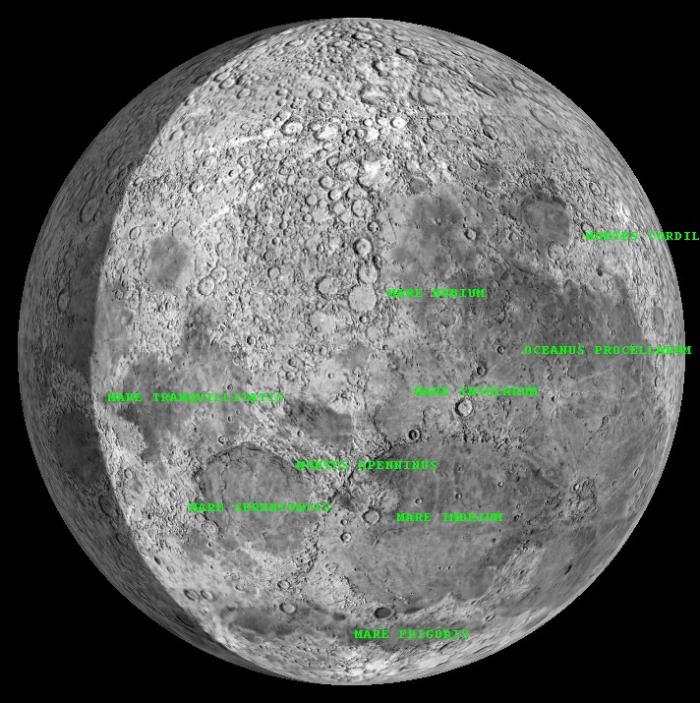
\includegraphics[width=.4\linewidth]{moon.png}
\end{minipage}%
\begin{minipage}{.333\textwidth}
  \centering
  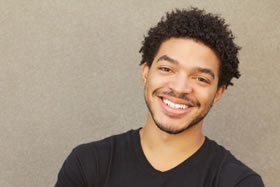
\includegraphics[width=.8\linewidth]{joshua.png}
\end{minipage}
\begin{minipage}{.333\textwidth}
  \centering
  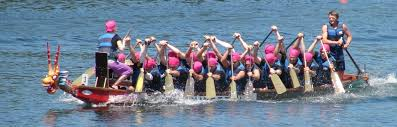
\includegraphics[width=.8\linewidth]{dragonboat.png}
\end{minipage}\\

Joshua has worked full-time for G-Research for 3 years now, and has been actively involved in graduate recruitment since working as a student ambassador following a summer internship. Joshua works as a Machine Learning Analyst, creating financial models to predict investment returns. Many of Joshua's colleagues have postgraduate degrees, however he recognises that mathematics and computing undergraduate students may have the required skills - in particular, the ability to independently implement theoretical ideas as working code. 

In his spare time, Joshua enjoys dragon boating along the Thames with friends from the office. Joshua also contributes to open source projects, for example a virtual moon atlas. Many students that Joshua meets at career fairs also pursue coding projects in their own time, however Joshua enjoys talking to any bright, enthusiastic and numerate student. Other than a few students that beeline to the G-Research stand, Joshua unfortunately finds it hard to attract attention, as most students flock to famous companies such as Google. When he does manage to attract a student's attention, he occasionally notices students queueing to talk with him, and then leaving before he gets the chance. 

\subsection{Nicolas}

\begin{minipage}{.333\textwidth}
  \centering
  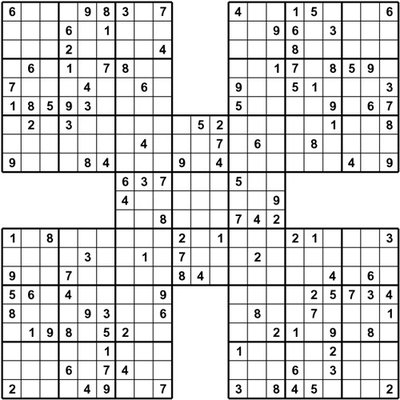
\includegraphics[width=.5\linewidth]{puzzle.png}
\end{minipage}%
\begin{minipage}{.333\textwidth}
  \centering
  
\includegraphics[width=.8\linewidth]{nicolas.png}
\end{minipage}
\begin{minipage}{.333\textwidth}
  \centering
  
\includegraphics[width=.5\linewidth]{hackathon.png}
\end{minipage}\\

Nicolas is a 3rd year BEng Computing student looking for a graduate role as a developer. He has a lot of programming experience from his degree, so finds it easy to work with new languages and get his head around complicated concepts. He could easily understand a simple API in a few minutes if it is well documented and intuitive. He enjoys puzzles and challenges and takes part in hackathons (such as Facebook Campus hackathons).

He plans to attend the Technology Careers Fair to find companies he would like to work at and apply to. He will attend the stalls of various well known companies, such as Google and Facebook. He is less inclined to talk with smaller companies unless their stand has a specific draw. Nicolas doesn't want to commit to being at a stand for long time, any activity that takes longer than 10 minutes might dissuade him from visiting a company. 

\section{Value Proposition Canvas}
We used our personas to create a Value Proposition Canvas that summarizes our understanding of the customer, the product we are producing and the explicit ways it is creating value for both G-Research and the students who will use it. It is clear that the gains/pains and their respective solutions, detailed below, are essentially hypotheses. As we moved forwards with user testing it was interesting to evaluate these proposed gain creators and pain relievers, and pivot development accordingly. We discuss our hallway testing later in the chapter (section 5.5). 

\subsection{Customer Segment}
\begin{tabularx}{\textwidth}{| c | X | X | X |}
	\hline
	& Customer Job(s) & Gains & Pains \\ 
	\hline\hline
	\multirow{4}{*}{Recruiter} & Advertise G-Research at  university careers fairs or special events
		       & Potential for fast tracking candidates 
		       & Not attracting candidates to G-Research stand at careers fair \\ \cline{2-4}

		       & Identify prospective employees
		       & Standing out at careers fairs among other companies, i.e. brand exposure
		       & Attracting unsuitable candidates \\ \cline{2-4}
	
		       & 
		       & Better understanding of what candidates look for when it comes to internships
		       & Generating too much attention to manage with only a few recruiters present \\ \cline{3-3}

		       & 
		       & Survey data about candidates, e.g. degree/year group
		       & \\ 
	
	\hline\hline
	\multirow{4}{*}{Student} & Learn about G-Research and its internship/graduate opportunities
		       & Enjoyable and informative conversation with recruiter from G-Research
		       & Waiting or not getting a chance to talk to a recruiter \\ \cline{2-4}

		       & If they like G-Research, apply for internship/graduate opportunities
		       & Contact details or application referral from recruiter
		       & Not learning enough about G-Research \\ \cline{2-4}

			&
			& Way of expressing programming/problem solving ability and impressing recruiter
			& Awkward conversation with a G-Research recruiter \\ \cline{3-4}
	
			&
			& 
			& Getting too much unwanted attention from a recruiter \\ \cline{4-4}

			&
			& 
			&  Unwanted pressure - feeling like performance/conversation is pivotal to application\\
	\hline
\end{tabularx}

\subsection{Value Proposition}
We can summarise our proposed product/service, before analysing how it influences our customers : 
\\[+1em]
\begin{tabular}{ r | l}
{\bf AI Racing Market} & Interactive multiplayer racing game \\
				   & Users compete by creating AI scripts\\
				   & Online code editor with javascript syntax highlighting \\
				   & User profiles with optional university/degree information \\
				   & Edit and test previous scripts \\
				   & Leaderboard system
\end{tabular} 
\\[+2em]
\begin{adjustbox}{center}
	\begin{tabularx}{\textwidth}{| c | X | X | X |}
	\hline
	& Gain Creators & Pain Relievers \\ 
	\hline\hline
	\multirow{4}{*}{Recruiter} 
		       & Candidates may become more relaxed and easier to talk to if enjoying the game
		       & Few recruiters go as far as having games at fairs, likely to attract interest \\ \cline{2-3}

		       & If candidates leave their email and produce good scripts, recruiters can get in contact with them
		       & Producing good AI requires logical problem solving, alongside programming skills which could be learnt by an inexperience but patient candidate - these candidates are likely appealing to G-Research\\ \cline{2-3}
	
		       & Recruiters can work with students and gave a genuine demonstration of how they work collaboratively/pair program at G-Research
		       & Large screen can show races, attracting spectators without forcing participation\\ 
	\hline\hline
\multirow{4}{*}{Student} 
		       & Can demonstrate both programming and logical problem solving skills to recruiter.
		       & Option to anonymously submit AI scripts, so there is no concern over AI performance being tracker and harming G-Research application\\ \cline{2-3}

		       & Can demonstrate teamwork skills if collaborating with other candidates
		       & Can collaborate with other students whilst waiting for a turn\\ \cline{2-3}

		       & May have positive experience developing iteratively with G-Research recruiter
		       & Recruiters are more likely free to talk if some candidates are busy playing game\\ \cline{2-3}
		       
		       & G-Research may award prizes for particularly impressive candidates
		       & Use of familiar programming language ({\tt javascript}) which also shouldn't punish inexperienced coders\\ 
	\hline
	\end{tabularx}
\end{adjustbox}


\section{Customer Feedback and Evaluation}
The primary point of contact with our customer, Ed, was a fortnightly sprint review meeting. These took place at the end of each sprint, allowing us to discuss progress made in the previous sprint and any expectations for the next one. To illustrate this let's examine a previous meeting:
\begin{enumerate}
\item First of all we set up a demo for the latest build of our project. Keeping a clean master branch for our stable code is critical for this, since we wouldn't want to be running around bug hunting just before Ed arrived.
\item After welcoming Ed to college, we ran through our new features on the demo, highlighting any user stories we successfully implemented. 
\item We explained any scoping decisions we had taken, such as pushing back user stories to the next sprint or pulling them forward. We were not afraid to take full advantage of Ed's knowledge as a developer, knowing he could understand some of the technical reasons behind the choices we'd made. 
\item  After this we passed the baton over to Ed, allowing him to offer any feedback on the features we'd implemented and discuss if he accepted the user stories as complete or still in need of work. He also discussed how the features fit into his vision of the final product, i.e. if we were making progress or racing off track. This feedback served as a last resort for keeping our goals aligned with our customer, preferably we would know if the feature fit into his vision before we began implementing it.
\item Once the evaluation stage was satisfied we discussed next week's sprint, in particular the stories he wanted us to work on. We divided these into requirements and stretch goals by estimating the development time required and the importance of the feature. Having this divide between stretch goals and requirements allowed us to balance our time appropriately, making sure we were steadily iterating towards a solid product while also able to add exciting, if not critical, features.
\item Finally we reviewed our progress in regards to the long term picture, considering how far we had made it towards the final product. We considered any features we would likely need to cut or add and planned around this appropriately.
\end{enumerate}

However, limiting contact time to once every two weeks is a dangerous trap to fall into; it would have left little room for us to maneuver around changing customer requirements or our own busy schedules. To help encourage continuous feedback throughout the project, we added Ed to our Trello board. This allowed him to keep track of our progress in between face-to-face meetings without adding extra communication overhead on our side. 

As for our communication needs, we could contact Ed in light of developing problems directly via email. One of such issues that arose was what environment we could expect our project to be running in - early in the project we had little knowledge of what technologies G-Research would be willing to support, making design decisions troublesome. It was critical that we got feedback from Ed immediately about what licenses and tools he'd be willing to burden. Leaving such discussions to the next meeting would have wasted huge amounts of development time in waiting, or scrapping unsuitable work.

On the other hand there are some discussions we could only have with Ed in the room. Some problems simply require throwing ideas back and forth, and the scripting language controlling our cars is a key example. Keeping the design of this approachable enough for a passing student while also offering depth enough for a particularly enthusiastic programmer is a risky balance. Too far one way and the challenge is dull and lifeless, while too far the other way and suddenly you have textbook sized instruction manuals and about one willing participant. The critical importance of this design was not lost on us, so customer feedback was crucial to our development process. Naturally, user testing (as we'll discuss shortly in section 5.5) also played a strong role in this.

To put it in development terms, continuous feedback from our customer for our evaluation process is similar to the continuous integration approach we used in our design process. Having these short cycles of work followed by review allowed us to iterate toward the end game without losing our focus or direction. Maintaining strong communication with our customer was essential to managing our requirements and at the end of the day, making sure we were implementing something our personas were going to want to use. 

\section{Managing and Prioritising Requirements}
After confirming, or adding, requirements during our customer meeting, the next task was to plan how we would tackle the requirements. As mentioned in the section above, we tried to find out during our meetings which features were the highest priority for the customer. This was a good starting point for our internal prioritisation and planning. After a customer meeting we tried to meet as a group to prune our product backlog and estimate the size and priorities of our stories for the coming sprint (backlog refinement). You might expect that this is an easy process, as we had found out feature priorities directly from our customer, however this was not the case. With new features it is very difficult to estimate their difficulty. This affects their priority as the amount of time a task takes affects how achievable they are within a tight timescale. 

A very easy mistake to make would be to jump straight into implementing a new exciting feature that was mentioned in a customer meeting. We avoiding falling into this trap by strictly following the task prioritisation as detailed on our Trello scrum board. For example, before attempting to implement turbo boosts we had to ensure users could edit their AI scripts. Our team may have spent days on implementing turbo boosts, slowly realising that it's a lot more of a challenge than we initially thought. By the end of the sprint, only half of the new feature may have been built, and the important changes to script editing may not have been made. Script editing is unexciting compared to power-ups, but without it a user's experience could be made difficult and our own testing would be slowed down.

\subsection{Timeboxed Spikes}
One of the mechanisms that we used to tackle this problem was the use of timeboxed spikes. There were several occasions in our project where we had difficulty in estimating how long a task would take and thus been apprehensive to begin their implementation. With these tasks it was useful to put some time aside for someone to jump in and see how feasible it is to complete. For example, during our penultimate sprint one of our tasks was to upgrade our racing AI API from a raycast system to a spline-following system. This change was designed to improve the smoothness of the car's movement and allow for our API to be more easily expanded and simplified. However, we were unsure of how easy this change would be and what benefits it would provide. Therefore, we set aside one afternoon for a member of the team to look into how the change would be made and begin its implementation. We decided that if no decent progress or results had been achieved during this time then we would not continue with the task. Luckily for us, we managed to get one racetrack working with the new system fairly quickly and found out that it did provide many benefits. We then went on to add full support for the system and implemented it on other racetracks.

\subsection{Prototypes}
Another thing that we used to ensure that we were spending our time on the right things was the use of paper prototypes. When developing new front end systems or features it can be a great time saver to nail down what you want a UI to look like before you begin working on it. Otherwise, a first iteration could be built and then when it's shown to a stakeholder, the design might turn out to be sub-optimal. The UI may then have to be rebuilt from scratch, in the worst case. Paper prototypes can be used to minimise this wasted time by getting feedback before any time has been spent building it. For example, here is a paper prototype that we used for the script submission page (from the perspective of an anonymous user):

\begin{center}
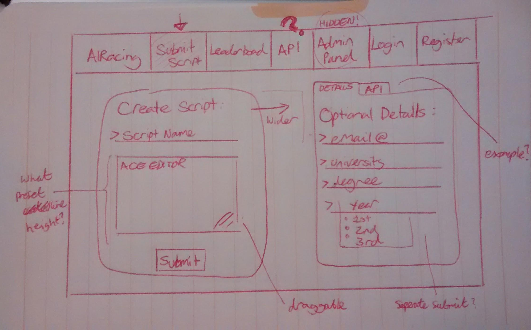
\includegraphics[scale=0.7]{mockup.png}
\end{center}

In our case this was simply used among our team to decide on a design. Which, while not as useful as getting direct customer feedback, allowed us to save time on any later redesigns due to any differences in the imagined look of the site between team members. 

From our experience using UI prototyping software such as Fluid UI, it is rigid and takes only a little less time to create a prototype than drafting up an actual web page. Paper prototypes give the impression that it is a work in process, whereas realistic prototypes can give the impression that too much time and effort has been vested in a UI for it to be changed. We consequently opted for paper prototyping to ensure we received honest feedback from Ed.

\section{Hallway Testing \bf NEEDS MAJOR WORK}
Hallway testing was our primary testing method since our target audience, Computing/Maths students, is too small to find reliable statistics through techniques such as the random sampling in A/B testing. Instead, we will setup a mock G-Research careers fair stand with one or two laptops. Our client and a colleague of his will invite students to write AI scripts, and we will assist where appropriate - we will minimise intervention.

We will encourage students to take around 5-10 minutes to write their scripts, as we believe this is representative of how long a student will have at a busy careers fair. Considering only a few laptops will be available, we will provide handouts containing an API reference, short tutorial and space for making notes. Whilst a student waits for a turn on the laptop, this will let them think about the problem and potentially discuss it with other candidates or the recruiters. We will not give the students any help unless required. We will hold regular tournaments during the test and ask students for feedback after submitting their scripts. 

Our primary goal is to promote G-Research, so our project should be exciting for students in order to draw more attention to their stand and consequently generate interest in G-Research. We will evaluate this by observing how much students engage with the game; ideally, there should be some competition to create the fastest script, with students returning to refine their scripts after they are pushed down on the leaderboard. Another key measure will be the time students stay at the stand: we know we need to improve our project if all students spend five minutes on the script and leave immediately afterwards, but we've accomplished this goal if students start asking for more time and stay to watch other scripts compete in tournaments.

After the testing, we will discuss how the game generated interest in G-Research with our client and his colleague. From their experience running careers fair stands, it is likely they will have a good idea of whether the software proved valuable as a means of connecting with prospective candidates, or whether it simply functioned as a fun distraction for students. 

An important goal of the project is the usability, as players will have limited means of learning the API given the unconventional setting of a careers fair. It is crucial that the API is easy to use with helpful tutorials and example/starter scripts. We can evaluate the usability by the quality of the scripts, for example, we know the tutorials or the API must be improved if most students submit simple low constant speed scripts or variations of the example scripts. We will ask students to rate the quality of the API, tutorials and example scripts after the test and combine this with our own insights from observing the test to evaluate the usability.

\section{Metrics \bf NEEDS MAJOR WORK}
Metrics are an important part of the feedback process. They will allow us to easily understand which parts of the workflow are going right and wrong, in order for us to improve working efficiency. They also allow us to see if our product is working as intended, and what parts need changing - either because they don't work or as part of general improvement.

\subsection{Workflow Metrics}
Our tasks on Trello currently have story points associated with them, which work as measures of task complexity. We can use this to graph how much work our team can complete in an average iteration, and see if there are any anomalies (which would probably be due to other coursework). We can also use this data to create burndown charts, which allows us to see whether we are going to complete our project on time or whether we will need to adjust our plan accordingly. 

\begin{center}
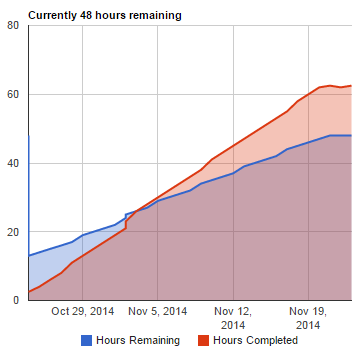
\includegraphics[scale=0.7]{burndown.png}
\end{center}

Creating this graph reveals an alarming trend of an increase in the number of hours remaining. However, this is due to the extra stories we bring into scope after our meetings with our customer go well - so it is not an immediate cause for concern. Reassuringly, our hours completed is fairly linear so we can clearly estimate how productive our team is each week. This makes planning for future weeks simpler as we have a strong idea of how much we can achieve (20 story points).

\subsection{Product Metrics}
We need to be able to evaluate how good a feature is, and quantitatively measure this so we can use it as feedback. There are a few methods for achieving this - for instance, for the website, we can record how long a user spends on a particular page, or how often they visit said page - this represents how popular the feature on the page is. 

It is also useful to determine what exactly users want, and whether we have provided that for them or not. This is usually best implemented as a search function, where we can then see what users searched for against what page they ended up with; however, since this feature isn't required for our product, we will instead have to use more direct methods such as user surveys, or perhaps a direct feature request button.

On this note, it would also be useful to determine which parts of the product the good candidates look at versus what parts everyone looks at, since this indicates what is interesting to the the type of people G-research want to hire, and means we can focus our development time on improving these parts in particular. For example, a strong candidate may take the time to fully understand the documentation, and would probably be able to improve on existing scripts easily.

We also need to know how interested people are in general - in this case it can be useful to determine how long a user spends against how long they want to spend. For this, we'd need a ratio of the total time spent at the stall and how long the spend writing/racing AI scripts - perhaps they'd want some time to speak to a recruiter but the time spent writing a script was so long they didn't really have a chance, or wanted to move on to other things.

The racing game is a good opportunity to record various statistics about the user. For instance, when starting the game, we can record which car models and racetracks are played the most, and how many players are commonly in one race. This is useful in deciding what the default settings should be, and also optimising the game for the most common amount of players.




\chapter{Conclusion}
\section{What did you learn? TODO: needs a bit more depth}

The length and depth of this project allowed us to learn a great many things,
consisting of new technologies and new work methodologies. Key to this is the
agile workflow, which was required for this project. We all learnt how using
agile methods can be better for quick prototyping and helping to focus our
project early through frequent refinement. This was also necessary when our
requirements changed throughout the project, which would've meant extensive
rework if we weren't using agile.

Some of the technologies new to us was the Unity game engine, which was required
to use for the racing simulation. Only one group member had previously used this
before, which helped a great deal with the initial work but other group members
had to learn the framework and its intricacies. 

We also had to learn Node.js and the Express framework, which made us deals with
a lot of asynchronous javascript callbacks, and the model view controller design
pattern. Whilst we have encountered some of this before, we now feel more
comfortable in this environment.

Working with MongoDB instead of an SQL database is also different, since we no
longer have relational databases and store most things in the same collection;
we managed to learn a bit more about the structure of NoSQL databases and how you
have to use them in a certain way that differs from what we are used to.

\section{What would we do differently? TODO}

We feel that a lot of our initial project work went well, with a protoype
quickly forming and features being organised quickly. Looking back now, it is
easy to judge the tasks that will be more important that we could've worked on
from the start, especially since G-Research have pointed out more of what they
want as the project went on. Most of what we did went well and worked for us, so
we wouldn't want to change how we worked drastically, but there were a few key
issues that would've resulted in fewer problems for us later.

One of these problems was with deploying the Unity side of the game. The
compiled web build had to be made with the Unity editor, and so was included in
the git repository as this is what was transferred to the VM our project ran on.
This web build was very large, and resulted in significantly long build times,
as well as causing us problems with disk space on the VM, since git would keep
all previous versions of it as part of its history. Towards the end of the
project, we found that there were ways of removing this build from previous
commits, which would help with our disk space problems. We also managed to find
a command line version of Unity that could compile the web build on the VM,
although this would have to run on Windows, whether through another virtual
machine or just having the one we used as Windows instead of Linux. We didn't
change this around as we had almost finished, and it could potentially break our
project at an important time if we tried to alter this too much. However, this
would be something we would strongly consider doing were we to do it again,
since it would solve a vast amount of the annoyances we encountered above.

Another problem was using the MongoDB database, although mostly at our own
fault. We made some initial collections that we thought would be separate, but
found later that we needed to 'join' them. However, this cannot be done easily
with NoSQL, and eventually we created a new collection to house all the data. We
felt slighly uncomfortable using something that didn't have relational data, and
never really got used to the paradigm shift, so perhaps using a relational model
would've sped up our working and avoided these problems. At the same time, it is
good to know about NoSQL databases, and we would not have learnt about it during
this project otherwise, so we would need to consider which tradeoffs are worth
it.
 
\begin{itemize}
    \item
        Try and stick better to agile?
    \item
        Try and get more frequent feedback (smaller sprints?)
    \item
        Testing
    \item
        Do more feedback sessions with users, i.e. do a few practice runs with
        groups of students to see if it's working well
\end{itemize}

\section{Future extensions}
% There can probably be a lot for this... list the key features we would
% want to add, or the ones we were planning on adding before we ran out of time

Whilst we got the key features completed on time, there are a few things we were 
thinking about doing towards the end of the project that we could do if we had
more time to work on it. G-Research have mentioned that this project could
potentially be continued by another university, so these extensions could
eventually form a specification for them to work on.

Below is a list of the extensions ideas we have and the reasons for them:

\begin{itemize}
    \item
        \textbf{More Extensive API} - Allowing more control over the car allows
        for more complex and detailed AI scripts, and could help find the best
        candidates who can use all the features. Examples of this include 
    \item
        \textbf{Better car physics} - Our simulated car physics could do with
        some improvements - for example when moving backwards the car has a
        tendency to flip over for no reason. The brake system also doesn't work
        that well with the road, meaning a negative throttle is more effective
        at stopping than braking is.
    \item
        \textbf{Cleaner setup} - Currently our deployment system consists of
        downloading the Github repository, and making sure to install the
        prerequisites (MongoDB and Node), then running the web server. This
        could be packaged up into an installer that bundles the compiled code
        and the prerequisites together for easy installation.
    \item
        \textbf{Better security} - We don't have much security for our project,
        mainly because it was only required to run at a careers fair in a closed
        network, which wouldn't be vulnerable anyway. However, those with
        knowledge of the source code could potentially use it to their advantage
        and modify the rules of the simulation, allowing them to perform better.
    \item
        \textbf{Better documentation} - More extensive documentation along with
        some example scripts on how to use the API would definitely aid future
        users with how best to go about writing a racing AI.
    \item
        \textbf{Improving other scripts} - this was originally part of the
        original specification, which wanted us to allow new players to see
        existing code and tweak it for better performance. We decided against
        this after we found this would be used at careers fairs to test
        candidates, as this would be unfair to the original authors of the
        scripts, and may lead to unfair perfomance comparisons.
        However, if the project were to be converted to more of a market than a
        performance tool, then this could then be integrated.
\end{itemize}



\section{Final words TODO}


\chapter{Bibliography}
\printbibliography[heading=none]

\appendix
\chapter{Appendix}
\section{ER Diagram}

\begin{center}
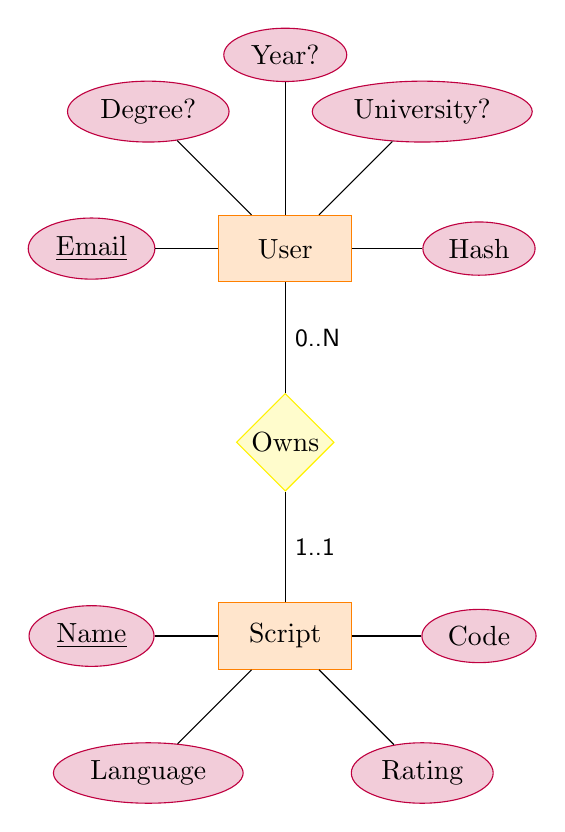
\begin{tikzpicture}[node distance=7 em]
\node [entity] (person) {User};
\node [relationship] (has) [below of=person] {Owns};
\node [entity] (script) [below of=has] {Script};
\node [attribute] (email) [left of=person] {\key{Email}} edge (person);
\node [attribute] (pid) [above of=person] {Year?} edge (person);
\node [attribute] (pid) [above left of=person] {Degree?} edge (person);
\node [attribute] (pid) [above right of=person] {University?} edge (person);
\node [attribute] (pid) [right of=person] {Hash} edge (person);
\node [attribute] (pid) [left of=script] {\key{Name}} edge (script);
\node [attribute] (pid) [right of=script] {Code} edge (script);
\node [attribute] (pid) [below left of=script] {Language} edge (script);
\node [attribute] (pid) [below right of=script] {Rating} edge (script);
%Edge
\path[every node/.style={font=\sffamily\small}] (person) edge node [right] {0..N} (has);
\path[every node/.style={font=\sffamily\small}] (script) edge node [right] {1..1} (has);
\end{tikzpicture}
\end{center}

\section{Instruction Manual}


\end{document}  
